\documentclass{jknotes}
\usepackage{../joshkirklin}
\usepackage{siunitx}
\usepackage{starfont}

\DeclareSIUnit\erg{erg}

\setmathfont{Latin Modern Math}
\setmathfont{GFS NeoHellenic Math}[range=bfsfup/{greek,Greek}->it]
\setmathfont{GFS NeoHellenic Math}[range=sfup/{latin,Latin}->it]

\newcommand{\B}{\symbf{B}}
\renewcommand{\u}{\symbf{u}}
\newcommand{\flux}{\symbf{\Phi}}
\newcommand{\disp}{\symbf{\xi}}
\renewcommand{\v}{\symbf{v}}
\newcommand{\dif}[1]{\left[#1\right]_1^2}
\newcommand{\M}{\mathcal{M}}

\usetikzlibrary{shapes.misc}

\tikzset{cross/.style={cross out, draw=black, minimum
size=2*(#1-\pgflinewidth), inner sep=0pt, outer sep=0pt}}
%default radius will be 1pt. 

\newcommand{\myol}[2][3]{{}\mkern#1mu\overline{\mkern-#1mu#2}}

\begin{document}

\institution{Cambridge Part III Maths}
\title{Astrophysical Fluid Dynamics}
\lecturer{Dr. Gordon Ogilvie}
\notetaker{Charles Powell}
\date{Lent 2020}

\maketitle
\suggestionsspiel
\tableofcontents

\lecture{22/01/21}
\section{Introduction}
\subsection{Areas of application}
Astrophysical fluid dynamics (AFD) is relevant to the description of the interiors
of stars and planets, exterior phenomena such as discs, winds and jets, the
interstellar medium, the intergalactic medium, and cosmology itself. A fluid
description is not applicable in regions that are solidified, such as the
rocky or icy cores of giant planets and the crusts of neutron stars, and also
in very genuous regions where the medium is not sufficiently collisional.

\subsection{Theoretical varieties}
Various flavours of AFD are in use. The basic models we will consider are:
\paragraph{Hydrodynamics (HD) / Newtonian gas dynamics:}
This model is non-relativistic, compressible, ideal (inviscid and adiabatic),
self-gravitating, and usually assumes a perfect gas.
\paragraph{Magnetohydrodynamics (MHD):}
This model is the same as above, with the addition of a magnetic field. We
will often use ideal MHD, which assumes a perfectly conducting fluid.

\subsection{Characteristic features}
The elements of theory often important in AFD are compressibility,
gravitation, and thermal physics. Sometimes, magnetic fields, radiation
forces, and relativity are important. Rarely important aspects are viscosity,
surface tension, and solid boundaries.

\subsection{Useful data}
Some useful data for the course, in CGS (centimetres, grams, seconds) units:
\begin{table}[h]
\begin{tabular}{ll}
	Newton's constant & $G = 6.674 \times 10^{-8} \,\si{\cm^3.\g^{-1}.\s^{-2}}$ \\
	Boltzmann's constant & $k = 1.381 \times 10^{-16} \, \si{\erg.\K^{-1}}$ \\
	Stefan's constant & $\sigma = 5.670 \times 10^{-5}
	\,\si{\erg.\cm^{-2}.s^{-1}.K^{-4}}$\\
	Speed of light & $c = 2.998 \times 10^{1-} \,\si{\cm.s^{-1}}$\\
	Hydrogen mass & $m_H = 1.674 \times 10^{-24} \, \si{\g}$\\
	Solar mass & $M_\Sun = 1.988 \times 10^{33} \,\si{\g}$\\
	Solar radius & $R_\Sun = 6.957 \times 10^{10} \, \si{\cm}$\\
	Solar luminosity & $L_\Sun = 3.828 \times 10^{33} \, \si{\erg \s^{-1}}$\\
	Parsec & $pc = 3.086 \times 10^{18} \, \si{\cm}$\\
	Astronomial unit (AU) & $au = 1.496 \times 10^{13} \, \si{\cm}$\\
	Joule erg conversion & $1 \si{\J} = 10^7 \si{\erg}$
\end{tabular}
\end{table}

\section{Ideal gas dynamics}
\subsection{Fluid variables}
A fluid is characterised by a velocity field $\symbf{u}(\symbf{x},t)$ and two
independent thermodynamic properties. Most useful are the dynamical variables:
the pressure $p(\symbf{x},t)$ and the mass density $\rho(\symbf{x},t)$. Other
properties, e.g. temperature $T$, can be regarded as functions of $p$ and
$\rho$. The \emph{specific volume} (volume per unit mass) is $v = 1/\rho$. 

We neglect the possible complications of variable chemical composition
associated with chemical and nuclear reactions, ionisation and recombination.

\subsection{Eulerian and Lagrangian viewpoints}
In the \emph{Eulerian} viewpoint we consider how fluid properties vary in time
at a point which is fixed in space, i.e. attached to the (usually inertial)
coordinate system. The Eulerian time derivative is simply $\partial_t$.

In the \emph{Lagrangian} viewpoint we consider how fluid properties vary in
time at a point which moves with the fluid at velocity
$\symbf{u}(\symbf{x},t)$. The Lagrangian time derivative (or material
derivative) is
\begin{equation}
	\frac{\diffD}{\diffD t} = \frac{\partial}{\partial t} +
	\symbf{u}\cdot\nabla
\end{equation}

\subsection{Material points and structures}
A material point is an idealised fluid element, a point that moves with the
bulk velocity $\symbf{u}(\symbf{x},t)$ of the fluid. Note that the true
particles of which the fluid is composed also have random thermal motion.

Material curves, surfaces and volumes are geometrical structures composed of
fluid elements; they move with the fluid flow and are deformed by it. An
infinitesimal material line element $\delta\symbf{x}$ evolves according to
\begin{equation}
	\frac{\diffD \delta \symbf{x}}{\diffD t} = \delta \symbf{u} =
	\delta\symbf{x}\cdot\nabla\symbf{u}
\end{equation}
It changes its length and/or orientation in the presence of a velocity
gradient.

Infinitesimal material surface or volume elements can be defined from two or
three material line elements according to the vector product and the triple
scalar product.
\begin{align}
	\delta \symbf{S} &= \delta \symbf{x}^{(1)} \times \delta \symbf{x}^{(2)} \\
	\delta V &= \delta \symbf{x}^{(1)} \cdot \delta \symbf{x}^{(2)} \times
	\delta \symbf{x}^{(3)}
\end{align}
They evolve according to
\begin{align}
	\frac{\diffD \delta \symbf{S}}{\diffD t} &= (\nabla \cdot \symbf{u})\delta
	\symbf{S} - \nabla \symbf{u} \cdot\delta \symbf{S}\\
	\frac{\diffD \delta V}{\diffD t} &= (\nabla \cdot \symbf{u})\delta V
\end{align}
The second result is easier to understand: the volume element increases when
the flow is divergent.

\subsection{Equation of mass conservation}
The equation of mass conservation
\begin{equation}
	\frac{\partial \rho}{\partial t} + \nabla \cdot (\rho \symbf{u}) = 0
\end{equation}
has typical form of conservation law: rate of change of a density and
divergence of a flux. Here, $\rho$ is mass density and $\rho \symbf{u}$ is mass
flux density.  An alternative form of the same equation is
\begin{equation}
	\frac{\diffD \rho}{\diffD t} = - \rho \nabla \cdot \symbf{u}
\end{equation}
If $\delta m = \rho \delta V$ is a material mass element, it can be seen that
mass is conserved in the form
\begin{equation}
	\frac{\diffD \delta m }{\diffD t} = 0
\end{equation}

\subsection{Equation of motion}
The equation of motion
\begin{equation}
	\rho \frac{\diffD \symbf{u}}{\diffD t} = - \rho \nabla \Phi - \nabla p
\end{equation}
derives from Newton's second law per unit volume with gravitational and
pressure forces. The gravitational potential is $\Phi(\x,t)$ and $\symbf{g} =
-\nabla\Phi$ is the gravitational field.

The force due to pressure acting on a volume $V$ with bounding surface $S$ is
\begin{equation}
	-\int_S p\, \diffd \symbf{S} = \int_V (-\nabla p) \, \diffd V
\end{equation}
Viscous forces are neglected in ideal gas dynamics.

\subsection{Poisson's equation}
The gravitational potential is related to the mass density by Poisson's
equation
\begin{equation}
\nabla^2 \Phi = 4\pi G \rho
\end{equation}
where $G$ is Newton's constant. The solution
\begin{equation}
	\Phi = \Phi_{\text{int}} + \Phi_{\text{ext}} = - G \int_V
	\frac{\rho(\x',t)}{\abs{\x'-\x}} \, \diffd^3 \x' - G \int_{\hat{V}} 
	\frac{\rho(\x',t)}{\abs{\x'-\x}} \, \diffd^3 \x' 
\end{equation}
generally involves contributions form both the fluid region $V$ under
consideration and the exterior region $\hat{V}$. A \emph{non-self-gravitating}
fluid is one of negligible mass for which $\Phi_{\text{int}}$ can be
neglected. More generally, the \emph{Cowling approximation} consists of
treating $\Phi$ as being specified in advance, so that Poisson's equation is
not coupled to the other equations.

\subsection{Thermal energy equation and equation of state}
In the absence of non-adiabatic heating (e.g. by viscous dissipation or
nuclear reactions) and cooling (e.g. by radiation or conduction),
\begin{equation}
	\frac{\diffD s}{\diffD t} = 0
\end{equation}
where $s$ is the \emph{specific entropy} (entropy per unit mass). Fluid
element undergo reversible thermodynamic changes and preserve their entropy
(adiabatic flow). This condition is violated in shocks (see section 6).

The thermal variables $(T,s)$ can be related to the dynamical variables
$(P,\rho)$ via an \emph{equation of state} and standard thermodynamic
identities. The most important case is that of an \emph{ideal gas} with
\emph{blackbody radiation}
\begin{equation}
	p = p_g + p_r = \frac{k \rho T}{\mu m_H} + \frac{4\sigma T^4}{3c}
\end{equation}
where $k$ is Boltzmann's constant, $m_H$ is mass of a hydrogen atom, $\sigma$
is Stefan's constant, $c$ is the speed of light, and $\mu$ is the mean
molecular weight, defined as the average mass of the particles in units of
$m_H$, equal to
\begin{itemize}
	\item $2.0$ for molecular hydrogen
	\item $1.0$ for atomic hydrogen
	\item $0.5$ for fully ionised hydrogen
	\item about $0.6$ for ionised matter of typical cosmic abundances.
\end{itemize}
The component $p_g$ is the \emph{gas pressure} and $p_r$ is the
\emph{radiation pressure}. Radiation pressure is usually negligible except in
the centres of high mass stars and in the immediate environments of neutron
stars and black holes. The pressure of an ideal gas is often written in the
form $\mathcal{R}\rho T/\mu$ where $\mathcal{R} = k/m_H$ is a version of the
universal gas constant.

We define the \emph{first adiabatic exponent}
\begin{equation}
	\Gamma_1 = \left( \frac{\partial \log p}{\partial \log \rho}\right)_S
\end{equation}
which is related to the ratio of specific heat capacities
\begin{equation}
	\gamma = \frac{c_p}{c_v} = \frac{T \left(\frac{\partial s}{\partial
	T}\right)_p}{T \left( \frac{\partial s}{\partial T}\right)_V}
\end{equation}
by $\Gamma_1 = \chi_\rho \gamma$ where
\begin{equation}
	\chi_\rho = \left( \frac{\partial \log p}{\partial \log \rho}\right)_T
\end{equation}
can be found from the equation of state. We can then rewrite the thermal
energy equation as
\begin{equation}
	\frac{\diffD p}{\diffD t} = \frac{\Gamma_1 p}{\rho} \frac{\diffD
	\rho}{\diffD t} = - \Gamma_1 p \nabla \cdot \symbf{u}
\end{equation}

For an ideal gas with negligible radiation pressure, $\chi_\rho =1$ and so
$\Gamma_1 = \gamma$. Adopting this very common assumption, we write
\begin{equation}
	\frac{\diffD p}{\diffD t} = -\gamma p \nabla \cdot \symbf{u}
\end{equation}

\subsection{Simplified models}
A \emph{perfect gas} may be defined as an ideal gas with constant $c_v, c_p,
\gamma$ and $\mu$. Equipartition of energy for a classical gas with $n$
degrees of freeodm per particle gives
\begin{equation}
	\gamma = 1 + \frac{2}{n}
\end{equation}

For a classical monatomic gas with $n=3$ translational degrees of freedom,
$\gamma = 5/3$. This is relevant for fully ionised matter. For a classical
diatomic gas with two addditional rotational degrees of freeodm, $n=5$ and
$\gamma = 7/5$. This is relevant for molecular hydrogen. In reality,
$\Gamma_1$ is variable when the gas undergoes ionisation or when the gas and
radiation pressures are comparable. 

The specific \emph{internal energy} (or \emph{thermal energy}) of a perfect
gas is
\begin{equation}
	e = \frac{p}{(\gamma-1)\rho} = \frac{n}{\mu m_H} \frac{1}{2}kT
\end{equation}
Note that each particle has an internal energy of $\frac{1}{2}kT$ per degree
of freedom, and the number of particles per unit mass is $1/{\mu m_H}$.

A \emph{barotropic} fluid is an idealised situation in which the relation $p(\rho)$
is known in advance. We can then dispense with the thermal energy equation.
For example, if the gas is strictly isothermal and perfect, $p = c_s^2 \rho$
with the constant $c_s$ being the isothermal sound speed. Alternatively, if
the gas is strictly homentropic (constant $s$) and perfect, then $p = K
\rho^\gamma$ with $K$ constant. 

An \emph{incompressible} fluid is an idealised situation in which
$\frac{\diffD \rho}{\diffD t} = 0$, implying $\nabla \cdot \symbf{u} = 0$.
This can be achieved formally by taking the limit $\gamma \to \infty$. The
approximation of incompressibility eliminates acoustic phenomena from the
dynamics. The ideal gas law itself is not valid at very high densities or
where quantum degeneracy is important.

\subsection{Microphysical basis}
It is useful to understand the way in which the fluid-dynamical equations are
derived microphysical considerations. The simplest model involves identical
neutral particles of mass $m$ of negligible size with no internal degrees of
freedom.

\subsubsection{Boltzmann equation}
Between collisions, particles follow Hamiltonian trajectories in their six
dimensional $(\x, \symbf{v})$ phase space:
\begin{equation}
	\dot{x}_i = v_i, \hspace{2em} \dot{v}_i = a_i - \frac{\partial
	\Phi}{\partial x_i}
\end{equation}

The distribution funnction $f(\x, \symbf{v},t)$ specifies the number density
of particles in phase space. The velocity moments of $f$ define the number
$n(\x,t)$ in real space, the bulk velocity $\symbf{u}(\x,t)$ and the velocity
dispersion $c(\x,t)$ according to
\begin{align}
	\int f \, \diffd^3 \symbf{v} &= n\\
	\int \symbf{v} f \, \diffd^3 \symbf{v} &= n \symbf{u} \\
	\int \abs{\symbf{v}-\symbf{u}}^2 f \, \diffd^3 \symbf{v} &= 3nc^2
\end{align}
Equivalently,
\begin{equation}
	\int v^2 f \, \diffd^3 \symbf{v} = n (\symbf{u}^2 + 3c^2)
\end{equation}
The relation between velocity dispersion and temperature is $kT = mc^2$. In
the absence of collisions, $f$ is conserved following the Hamiltonian flow in
phase space. This is because particles are conserved and the flow in phase
space is incompressible. More generally, $f$ evolves according to
\emph{Boltzmann's equation}
\begin{equation}
	\frac{\partial f}{\partial t} + v_j \frac{\partial f}{\partial x_j} + a_j
	\frac{\partial f}{\partial v_j} = \left( \frac{\partial f}{\partial
	t}\right)_c
\end{equation}

The collision term on the RHS is a complicated integral operator but has 3
simple properties corresponding to the conservation of mass, momentum and
energy in collisions.
\begin{align}
	\int m \left( \frac{\partial f}{\partial t}\right)_c \, \diffd^3 \symbf{v}
	&= 0 \\
	\int m \symbf{v}\left( \frac{\partial f}{\partial t}\right)_c \, \diffd^3 \symbf{v}
	&= 0 \\
	\int \frac{1}{2}m\symbf{v}^2 \left( \frac{\partial f}{\partial t}\right)_c \, \diffd^3 \symbf{v}
	&= 0
\end{align}
The collision term is local in $\x$ (not even involving derivatives) although
it does involve integrals over $\symbf{v}$. The equation $\left(\frac{\partial
f}{\partial t}\right)_c = 0$ has the general solution
\begin{equation}
	f = f_M = (2\pi c^2)^{-3/2} n \exp\left( -
	\frac{\abs{\symbf{v}-\symbf{u}}^2}{2c^2}\right)
\end{equation}
with parameters $n, \symbf{u}$ and $c$ that may depend on $\x$. This is the
\emph{Maxwellian distribution}. 

\subsubsection{Derivation of fluid equations}
A crude but illuminating model of the collision operator is the \emph{BGK
approximation}
\begin{equation}
	\left( \frac{\partial f}{\partial t}\right)_c \approx - \frac{1}{\tau}
	(f-f_M)
\end{equation}
where $f_M$ is a Maxwellian distribution with the same $n, \symbf{u}$ and $c$
as $f$, and $\tau$ is the \emph{relaxation time}. This timescale $\tau$ can be
identified approximately with the mean flight time of particles between
collisions. The collisions attempt to restore a Maxwellian distribution on a
characteristic timescale $\tau$. They do this by randomising the particle
velocities in a way consistent with the conservation of momentum and energy.
If the characteristic timescale of the fluid flow is much greater than $\tau$,
then the collision term dominates the Boltzmann equation and $f$ is very close
to $f_m$. This is the \emph{hydrodynamic limit}. 

The velocity moments of $f_M$ can be determined from standard Gaussian
integrals, in particular
\begin{align}
	\int f_M \, \diffd^3 \symbf{v} &= n \\
	\int v_i f_M \, \diffd^3 \symbf{v} &= n u_i \\
	\int v_i v_j f_M \, \diffd^3 \symbf{v} &= n(u_i u_j + c^2 \delta_{ij}) \\
	\int \symbf{v}^2 v_i f_M \, \diffd^3 \symbf{v} &= n(\symbf{u}^2 + 5 c^2)
	u_i
\end{align}
We obtain equations for mass, momentum and energy by taking moments of the
Boltzmann equation weighted by $(m, mv_i, \frac{1}{2}m\symbf{v}^2)$. In each
case the collision term integrates to $0$ because of its conservative
properties, and the $\partial/\partial v_j$ term can be integrated by parts.
We replace $f$ with $f_M$ when evaluating the LHS and note that $mn = \rho$:
\begin{align}
	\frac{\partial \rho}{\partial t} + \frac{\partial}{\partial x_i} (\rho u_i) &= 0 \\
	\frac{\partial}{\partial t}(\rho u_i) + \frac{\partial}{\partial x_j}
	\left[ \rho (u_i u_j + c^2 \delta_{ij})\right] - \rho a_i &= 0 \\
	\frac{\partial}{\partial t} \left[\frac{1}{2}\rho \symbf{u}^2 + \frac{3}{2}\rho
	c^2\right] + 
	\frac{\partial}{\partial x_i} \left[ (\frac{1}{2}\rho \symbf{u}^2 +
	\frac{5}{2}\rho c^2) u_i\right] - \rho u_i a_i &= 0
\end{align}

These are equivalent to the equations of ideal gas dynamics in conservative
form (see section 4) for a monatomic ideal gas ($\gamma = 5/3$). The specific
internal energy is $\rho = \frac{3}{2}c^2 = \frac{3}{2}\frac{kT}{m}$.

\subsection{Validity of fluid approach}
Deviations from Maxwellian distribution are small when collisions are frequent
compared to the characteristic timescale of the flow. In higher-order
approximations these deviations can be estimated, leading to the equations of
dissipative gas dynamics including transport effects (viscosity and heat
conduction). 

The fluid approach breaks down if the mean flight time $\tau$ is
not much less than the characteristic timescale of the flow, or if the mean
free path $\lambda \approx c \tau$ between collisions is not much less than
the characteristic lengthscale of the flow.

The Coulomb cross-section for `collisions' (i.e. large-angle scatterings)
between charged particles (electrons or ions) is
\begin{equation}
	\sigma \approx 1 \times 10^{-4} (T/K)^{-2} \text{cm}^2
\end{equation}
The mean free path is $\lambda = 1/n\sigma$.

\section{Ideal magnetohydrodynamics}

\subsection{Elementary derivation of MHD equations}
\emph{Magnetohydrodynamics} (MHD) is the dynamics of an electrically
conducting fluid (a full or partially ionised gas or a liquid metal)
containing a magnetic field. It is a fushion of fluid dynamics and
electromagnetism.

\subsubsection{Galilean electromagnetism}
The equations of Newtonian gas dynamics are invariant under the Galilean
transformation to a frame of reference moving with uniform velocity
$\symbf{v}$,
\begin{equation}
	\symbf{x}'=\symbf{x}-\symbf{v}t, \hspace{1em} t' = t
\end{equation}

Under this change of frame, the fluid velocity transforms according to
\begin{equation}
	\symbf{u}'=\symbf{u}-\symbf{v}
\end{equation}
while scalar variables such as $p, \rho$, and $\Phi$ are invariant. The
Lagrangian time derivative $\diffD/\diffD t$ is also invariant, because the
partial derivatives transform according to
\begin{equation}
	\nabla' = \nabla, \hspace{1em} \frac{\partial}{\partial t'} =
	\frac{\partial}{\partial t} + \symbf{v}\cdot\nabla
\end{equation}

To derive a consistent Newtonian theory of MHD, valid for situations in which
the fluid motions are slow compared to the speed of light, we use Maxwell's
equations without the displacement current:
\begin{align}
	\frac{\partial \symbf{B}}{\partial t} &= - \nabla \times \symbf{E} \\
	\nabla \cdot \symbf{B} &= 0 \\
	\nabla \times \symbf{B} &= \mu_0 \symbf{J}
\end{align}
We will not require the fourth Maxwell equation, involving $\nabla \cdot
\symbf{E}$, because the charge density will be found to be unimportant. The
equation of energy conservation is
\begin{equation}
	\frac{\partial}{\partial t} \left( \frac{B^2}{2\mu_0}\right) + \nabla
	\cdot \left( \frac{\symbf{E}\times\symbf{B}}{\mu_0}\right) = -
	\symbf{E}\cdot\symbf{J}
\end{equation}
in which the energy density $B^2/2\mu_0$ is purely magnetic, while the energy
flux density has the usual form of the \emph{Poynting vector}
$\symbf{E}\times\symbf{B}/\mu_0$. These `pre-Maxwell' equations are invariant
under the Galilean transformation, provided that the fields transform
according to
\begin{equation}
	\symbf{E}'=\symbf{E}+\symbf{v}\times\symbf{B}, \hspace{1em}
	\symbf{B}'=\symbf{B}, \hspace{1em} \symbf{J}'=\symbf{J}
\end{equation}

\subsubsection{Induction equation}
In the \emph{ideal MHD approximation} we regard the fluid as a perfect
electrical conductor. The electric field in the rest frame of the fluid
therefore vanishes, implying that
\begin{equation}
	\symbf{E} = - \symbf{u}\times\symbf{B}
\end{equation}
in a frame in which the fluid velocity is $\symbf{u}(\x,t)$. This condition
can be regarded as the limit of a constitutive relationship such as Ohm's law,
in which the effects of resistivity (i.e. finite conductivity) are neglected.
From Maxwell's equations, we then obtain the \emph{ideal induction equation}
\begin{equation}
	\frac{\partial \symbf{B}}{\partial t} = \nabla \times (\symbf{u} \times
	\symbf{B})
\end{equation}
This is an evolutionary equation for $\symbf{B}$ alone, having elimnated
$\symbf{E}$ and $\symbf{J}$. The divergence of the induction equation,
\begin{equation}
	\frac{\partial}{\partial t} \left( \nabla \cdot \symbf{B}\right) = 0
\end{equation}
ensures that $\symbf{B}$ remains solenoidal. 

\subsubsection{Lorentz force}
A fluid carrying a current density $\symbf{J}$ in a magnetic field $\symbf{B}$
experiences a Lorentz force
\begin{equation}
	\symbf{F}_m = \symbf{J} \times \symbf{B} = \frac{1}{\mu_0} (\nabla \times
	\symbf{B}) \times \symbf{B}
\end{equation}
per unit volume. This can be understood as the sum of the Lorentz forces on
individual particles of charge $q$ and velocity $\symbf{v}$,
\begin{equation}
	\sum q \symbf{v} \times \symbf{B} = \left(\sum q
	\symbf{v}\right)\times\symbf{B}
\end{equation}

The electrostatic force can be shown to be negligible in the Newtonian limit.
In Cartesian co-ordinates we have
\begin{align}
	(\mu_0 \symbf{F}_m)_i &= \varepsilon_{ijk}\varepsilon_{jlm}\frac{\partial
	B_m}{\partial x_l} B_k \\
					  &= \left( \frac{\partial B_i}{\partial x_k} -
					  \frac{\partial B_k}{\partial x_i} \right) B_k \\
					  &= B_k \frac{\partial B_i}{\partial x_k} -
					  \frac{\partial}{\partial x_i} \left(
					  \frac{B^2}{2}\right)
\end{align}
Thus the Lorentz force can be written as
\begin{equation}
	\symbf{F}_m = \frac{1}{\mu_0} \symbf{B}\cdot\nabla\symbf{B} - \nabla
	\left( \frac{B^2}{2\mu_0}\right)
\end{equation}
The first term can be interpreted as a \emph{curvature force} due to a
\emph{magnetic tension} $T_m = B^2/\mu_0$ per unit area in the field lines.
The second term is the gradient of an isotropic \emph{magnetic pressure} $p_m
= B^2/2\mu_0$ which is also the magnetic energy density. The magnetic tension
gives rise to \emph{Alfv\'{e}n waves} (see later), which travel parallel to
the magnetic field with characteristic speed
\begin{equation}
	v_a = \left(\frac{T_m}{\rho}\right)^{1/2} = \frac{B}{\sqrt{\mu_0 \rho}}
\end{equation}
the \emph{Alfv\'{e}n speed}, or (vector) \emph{Alfv\'{e}n velocity}
\begin{equation}
	\symbf{v}_a = \frac{\symbf{B}}{\sqrt{\mu_0 \rho}}
\end{equation}
The magnetic pressure also affects the propagation of sound waves, which
become \emph{magnetoacoustic waves} (see later). The combination
\begin{equation}
	\Pi = p + \frac{B^2}{2\mu_0}
\end{equation}
is often referred to as the \emph{total pressure}, while the ratio
\begin{equation}
	\beta = \frac{p}{B^2/2\mu_0}
\end{equation}
is known as the \emph{plasma beta}. 

\subsubsection{Summary of the MHD equations}
The full set of ideal MHD equations is
\begin{align}
	\frac{\partial \rho}{\partial t} + \nabla \cdot (\rho \symbf{u}) &= 0 \\
	\rho \frac{\diffD \symbf{u}}{\diffD t} &= - \rho \nabla \Phi - \nabla p +
	\frac{1}{\mu_0}(\nabla \times \symbf{B})\times\symbf{B} \\
	\frac{\diffD s}{\diffD t} &= 0 \\
	\frac{\partial \symbf{B}}{\partial t} &= \nabla \times (\symbf{u} \times
	\symbf{B}) \\
	\nabla \cdot \symbf{B} &= 0
\end{align}
together with the equation of state, Poisson's equation, etc., as required.
Most of these equations can be written in at least one other way that may be
useful in different circumstances.

\subsection{Physical interpretation of MHD}
There are two aspects to MHD:
\begin{itemize}
	\item Advection of $\symbf{B}$ by $\symbf{u}$ (induction equation)
	\item Dynamical back-reaction of $\symbf{B}$ on $\symbf{u}$.
\end{itemize}

\subsubsection{Kinematics of the magnetic field}
The ideal induction equation
\begin{equation}
	\frac{\partial \symbf{B}}{\partial t} = \nabla \times (\u \times
	\B)
\end{equation}
has a beautiful geometric interpretation: magnetic field lines are `frozen in'
to the fluid and can be identified with material curves. One way to show this
result is to use the identity
\begin{equation}
	\nabla \times (\u \times \B) = (\B \cdot \nabla)\u - \B(\nabla\cdot\u) -
	(\u\cdot\nabla)\B + \u(\nabla \cdot \B)
\end{equation}
to write the induction equation in the form
\begin{equation}
	\frac{\diffD \B}{\diffD t} = (\B \cdot \nabla) \u - \B (\nabla \cdot \u)
\end{equation}
and use the equation of mass conservation
\begin{equation}
	\frac{\diffD \rho}{\diffD t} = - \rho \nabla \cdot \u
\end{equation}
to obtain
\begin{equation}
	\frac{\diffD}{\diffD t} \left( \frac{\B}{\rho}\right) =
	\left(\frac{\B}{\rho}\right)\cdot\nabla\u
\end{equation}
This is exactly the same equation satisfied by a material line element
(section 2.3). Therefore a magnetic field line (an integral curve of
$\B/\rho$) is advected and distorted by the fluid in the same way as a
material curve. A complementary property is that the magnetic flux $\delta
\flux = \B \cdot \delta\symbf{S}$ through a material surface is conserved:
\begin{align}
	\frac{\diffD \flux}{\diffD t} &= \frac{\diffD \B}{\diffD t} \cdot \delta
	\symbf{S} + \B \cdot \frac{\diffD \delta \symbf{S}}{\diffD t} \\ 
								  &= \left( B_j \frac{\partial u_i}{\partial
								  x_j} - B_i \frac{\partial u_j}{\partial x_j}
								  \right) \delta S_i + B_i \left(
								  \frac{\partial u_j}{\partial x_j} \delta S_i
								  - \frac{\partial u_j}{\partial x_i} \delta
								  S_j\right) \\
								  &= 0
\end{align}
By extension, we have conservation of the magnetic flux $\flux = \int \B \cdot
\diffd \symbf{S}$ passing through any material surface.

\subsubsection{ (Partial) analogy with vorticity}
In homentropic (uniform entropy) or barotropic ideal fluid dynamics in the
absence of a magnetic field, the vorticity $\symbf{\omega} = \nabla \times \u$
satisfies
\begin{equation}
	\frac{\partial \symbf{\omega}}{\partial t} = \nabla \times (\u \times
	\symbf{\omega})
\end{equation}
Vortex lines are then `frozen in' to the fluid. Conserved quantity
\begin{equation}
	\int_S \symbf{\omega} \cdot \diffd \symbf{S} = \oint_C \u \cdot \diffd
	\x
\end{equation}
is analogous to
\begin{equation}
	\int_S \B \cdot \diffd \symbf{S} = \oint_C \symbf{A}\cdot\diffd \x
\end{equation}
However, $\symbf{\omega}$ and $\u$ are directly related by $\symbf{\omega} =
\nabla \times \u$ whereas in MHD $\B$ and $\u$ are indirectly related through
the equation of motion and the Lorentz force, so the analogy between vorticity
dynamics and MHD is limited in scope.

\subsubsection{Lorentz force}
The Lorentz force per unit volume, 
\begin{equation}
	\symbf{F}_m = \frac{1}{\mu_0} \B \cdot \nabla \B - \nabla (B^2/2\mu_0)
\end{equation}
can also be written as the divergence of the \emph{Maxwell stress tensor}
\begin{equation}
	\symbf{F}_m = \nabla \cdot \symsf{M}, \hspace{2em}\symsf{M} =
	\frac{1}{\mu_0} \left( \B \B - \frac{B^2}{2}\symsf{I}\right)
\end{equation}
where $\symsf{I}$ is the identity tensor. In Cartesian components,
\begin{equation}
	(\symbf{F}_m)_i = \frac{\partial \symsf{M}_{ji}}{\partial x_j},
	\hspace{2em} \symsf{M}_{ij} = \frac{1}{\mu_0} \left( B_i B_j -
	\frac{B^2}{2}\delta_{ij} \right)
\end{equation}
If $\B$ is locally aligned with the $x$-axis, then
\begin{equation}
	\symsf{M} = \begin{pmatrix} T_m & 0 & 0 \\ 0 & 0 & 0 \\ 0 & 0 & 0
		\end{pmatrix} - \begin{pmatrix} p_m & 0 &0  \\ 0 & p_m & 0 \\ 0 & 0 &
	p_m \end{pmatrix}
\end{equation}
showing the magnetic tension and pressure. Combining the ideas of magnetic
tension and a frozen-in field leads to the picture of field lines as elastic
strings embedded in the fluid. There is a close analogy between MHD and the
dynamics of polymer solutions. The magnetic field imparts elasticity to the
fluid.

\subsubsection{Differential rotation and torsional Alfv\'{e}n waves}
First consider the kinematic behaviour of a magnetic field in the presence of
a prescribed velocity field involving differential rotation. In cylindrical
polar coordinates $(r,\phi,z)$ let 
\begin{equation}
	\u = r \Omega(r,z) \hat{\symbf{\phi}}
\end{equation}
Consider an axisymmetric magnetic field, which we separate into
\emph{poloidal} (meridional: $r$ and $z$) and \emph{toroidal} (azimuthal:
$\phi$) parts:
\begin{equation}
	\B = \B_p(r,z,t) + B_\phi(r,z,t) \hat{\symbf{\phi}}
\end{equation}
The ideal induction equation reduces to
\begin{equation}
	\frac{\partial \B_p}{\partial t} = 0, \hspace{2em} \frac{\partial
	B_\phi}{\partial t} = r \B_p \cdot \nabla \Omega
\end{equation}
Differential rotation winds the poloidal field to generate a torsional field.
To obtain a steady state without winding, we require the angular velocity to
be constant along each magnetic field line:
\begin{equation}
	\B_p \cdot \nabla \Omega = 0
\end{equation}
a result known as \emph{Ferraro's law of isorotation}. 

There is an energetic cost to winding the field, as work is done against
magnetic tension. In a dynamical situation a strong magnetic field tends to
enforce isorotation along its length. Generalise the analysis to allow for
axisymmetric torsional oscillations:
\begin{equation}
	\u = r \Omega(r,z,t) \hat{\symbf{\phi}}
\end{equation}
The azimuthal component of the equation of motion is then
\begin{equation}
	\rho r \frac{\partial \Omega}{\partial t} = \frac{1}{\mu_09 r} \B_p \cdot
	\nabla( r \B_\phi)
\end{equation}
Combine with the induction equation above to give
\begin{equation}
	\frac{\partial^2 \Omega}{\partial t^2} = \frac{1}{\mu_0 \rho r^2} \B_p
	\cdot \nabla (r^2 \B_p \cdot \nabla \Omega)
\end{equation}
This equation describes \emph{torsional Alfv\'{e}n waves}. For example, if
$\B_p = B_z \hat{\symbf{z}}$ is vertical and uniform, then
\begin{equation}
	\frac{\partial^2 \Omega}{\partial t^2} = v_a^2 \frac{\partial^2
	\Omega}{\partial z^2}
\end{equation}
This is not strictly an exact non-linear analysis because we have neglected
the force balance (and indeed motion) in the meridional plane.

\subsubsection{Force-free fields}
In regions of low density, e.g. the solar corona, $\B$ may be dynamically
dominant over inertia, gravity and gas pressure. We then have (approximately)
a force-free magnetic field such that
\begin{equation}
	(\nabla \times \B) \times \B = 0
\end{equation}
Since $\nabla \times \B$ must be parallel to $\B$ in this case, we may write
\begin{equation}
	\nabla \times \B = \lambda \B
	\label{eq:1}
\end{equation}
for some scalar field $\lambda(\x)$. Taking the divergence of \eqref{eq:1}
gives
\begin{equation}
	0 = \B \cdot \nabla \lambda
\end{equation}
so $\lambda$ is constant along each magnetic field line. In the special case
where $\lambda$ is constant, known as a \emph{linear force-free magnetic
field}, the curl of \eqref{eq:1} results in the \emph{Helmholtz equation}
\begin{equation}
	-\nabla^2 \B = \lambda^2 \B
\end{equation}
which admits a wide variety of solutions. A subset of force-free magnetic
fields consists of \emph{potential} or \emph{current-free} magnetic fields for
which
\begin{equation}
	\nabla \times \B = 0
\end{equation}
In a true vacuum, $\B$ must be potential. However, only an extremely low
density of electrons is needed to make the force-free description more
relevant. 

An example of a force-free field in cylindrical polar coordinates $(r,\phi,z)$
is
\begin{align}
	\B &= B_\phi(r)\hat{\symbf{\phi}} + B_z(r)\hat{\symbf{z}} \\
	\nabla \times \B &= -\frac{\diffd B_z}{\diffd r} \hat{\symbf{\phi}} +
	\frac{1}{r}\frac{\diffd}{\diffd r}\left(rB_\phi\right)\hat{\symbf{z}}
\end{align}
Now $\nabla \times \B = \lambda \B$ implies
\begin{equation}
	-\frac{1}{r}\frac{\diffd}{\diffd r} \left( r \frac{\diffd B_z}{\diffd
	r}\right) = \lambda^2 B_z
\end{equation}
which is the $z$ component of the Helmholtz equation. The solution regular at
$r=0$ is
\begin{equation}
	B_z = B_0 J_0(\lambda r), \hspace{2em} B_\phi = B_0 J_1(\lambda r)
\end{equation}
where $J_n$ is the Bessel function of order $n$. Note that $J_0(x)$ satisfies
\begin{equation}
	(xJ_0')' + xJ_0 = 0, \hspace{2em} J_1(x) = -J_0'(x)
\end{equation}
The helical nature of this field is typical of force-free fields with $\lambda
\ne 0$.

\subsubsection{Magnetostatic equilibrium and magnetic buoyancy}
A \emph{magnetostatic equilibrium} is a static solution ($\u = 0$) of the
equation of motion, i.e. one satisfying
\begin{equation}
	0 = - \rho \nabla \Phi - \nabla p + \frac{1}{\mu_0} (\nabla \times \B)
	\times \B
\end{equation}
together with $\nabla \cdot \B = 0$. While solutions do exist, inhomogeneities
in $\B$ often result in a lack of equilibrium. A magnetic flux tube is an
idealised situation in which the magnetic field is localised to the interior
of a tube and vanishes outside.
\begin{center}
	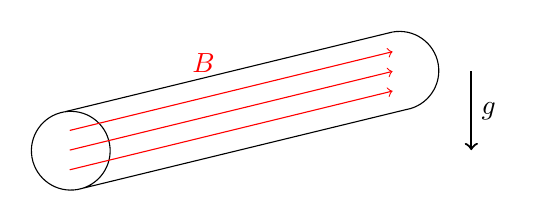
\begin{tikzpicture}
		\draw (-0.15,0.49) -- (4, 1.5);
		\draw (4,1.5) arc (100:-80:0.5) -- (0, -0.5) arc (-80:-440:0.5);
		\draw[red, ->] (-0.1, 0) -- (4, 1);
		\draw[red, ->] (-0.1, 0.25) -- (4, 1.25);
		\draw[red, ->] (-0.1, -0.25) -- (4, 0.75);
		\draw[thick,->] (5, 1) -- (5, 0) node[midway,right] {$g$};
		\draw[red] (1.6, 1.1) node {$\B$};
	\end{tikzpicture}
\end{center}

To balance the total pressure at the interface, the gas pressure must be lower
inside. Unless the temperatures are different, the density is lower inside. In
a gravitational field the tube experiences an upward buoyancy force and tends
to rise.

\section{Conservation laws \& hyperbolic structure}
\subsection{Introduction}
An equation in conservative form is written
\begin{equation}
	\frac{\partial q}{\partial t} + \nabla \cdot \symbf{F} = 0
\end{equation}
where $q(\x,t)$ is the density of some property and $\symbf{F}(\x,t)$ is the
flux density of the same quantity. The total amount in a time-independent
volume $V$ is
\begin{equation}
	Q = \int_V q \, \diffd V
\end{equation}
and evolves due to the flux through the bounding surface
\begin{equation}
	\frac{\diffd Q}{\diffd t} = - \int_V \nabla \cdot \symbf{F} \, \diffd V =
	- \int_S \symbf{F} \cdot \diffd \symbf{S}
\end{equation}
The prototypical choice for this equation is mass conservation with $q = \rho,
\symbf{F} = \rho \u$. 

A \emph{material invariant} is a scalar field $f(\x,t)$ for which
$\frac{\diffD f}{\diffD t} = 0$. Then $f$ is constant for each fluid element,
and is therefore conserved following the fluid motion. An example is specific
entropy $s$ in ideal fluid dynamics. Combined with mass conservation we obtain
an equation in conservative form:
\begin{equation}
	\frac{\partial}{\partial t}(\rho f) + \nabla \cdot (\rho f \u) = 0
\end{equation}

\subsection{Total energy equation}
Starting from the ideal MHD equations, we construct the total energy equation
piece by piece. First, consider \emph{kinetic energy}:
\begin{equation}
	\rho \frac{\diffD}{\diffD t}\left( \frac{1}{2}u^2\right) = \rho \u \cdot
	\frac{\diffD \u}{\diffD t} = - \rho \u \cdot \nabla \Phi - \u \cdot \nabla
	p + \frac{1}{\mu_0} \u \cdot (\nabla \times \B) \times \B
\end{equation}

\emph{Gravitational energy} (assuming a non-self-gravitating fluid and $\Phi$
independent of $t$):
\begin{equation}
	\rho \frac{\diffD \Phi}{\diffD t} = \rho \u \cdot \nabla \Phi
\end{equation}
\emph{Internal (thermal) energy} (using the fundamental thermodynamic identity
$\diffd e = T \diffd s - p \diffd v$):
\begin{equation}
	\rho \frac{\diffD e}{\diffD t} = \cancel{\rho T \frac{\diffD s}{\diffD t}}
	+ p \frac{\diffD \log \rho}{\diffD t} = - p \nabla \cdot \u
\end{equation}

Summing these three equations gives
\begin{equation}
	\rho \frac{\diffD}{\diffD t} \left( \frac{1}{2}\u^2 + \Phi + e\right) = -
	\nabla \cdot (p \u) + \frac{1}{\mu_0} \u \cdot (\nabla \times \B) \times
	\B
\end{equation}

Rewrite the Lorentz force term:
\begin{equation}
	\frac{1}{\mu_0} \u \cdot (\nabla \times \B) \times \B = \frac{1}{\mu_0}
	(\nabla \times \B) \cdot (-\u \times \B) = \frac{1}{\mu_0} (\nabla \times
	\B) \cdot \symbf{E}
\end{equation}

Using mass conservation:
\begin{equation}
	\frac{\partial}{\partial t} \left[ \rho (\frac{1}{2}\u^2 + \Phi +
	\rho)\right] + \nabla \cdot \left[ \rho \u (\frac{1}{2}\u^2 + \Phi + \rho)
	+ p \u\right] = \frac{1}{\mu_0} (\nabla \times \B) \cdot \symbf{E}
\end{equation}
Finally, consider the magnetic energy:
\begin{equation}
	\frac{\partial}{\partial t} \left( \frac{\B^2}{2\mu_0}\right) =
	\frac{1}{\mu_0} \B \cdot \frac{\partial \B}{\partial t} = -
	\frac{1}{\mu_0} \B \cdot (\nabla \times \symbf{E})
\end{equation}
The total energy equation is then
\begin{equation}
	\frac{\partial}{\partial t} \left[ \rho (\frac{1}{2}\u^2 + \Phi +
	\rho) + \frac{\B^2}{2\mu_0} \right] + \nabla \cdot \left[ \rho \u
	(\frac{1}{2}\u^2 + \Phi + h) + \frac{\symbf{E}\times\B}{\mu_0}\right] = 0
\end{equation}
where $h = e + p/\rho$ is the \emph{specific enthalpy} and we have used the
identity
\begin{equation}
	\nabla \cdot (\symbf{E} \times \B) = \B \cdot \nabla \times \symbf{E} -
	\symbf{E} \cdot \nabla \times \B
\end{equation}
to include the \emph{Poynting vector} (EM energy flux density)
$\symbf{E}\times \B / \mu_0$. The total energy is therefore conserved.

For a self-gravitating system satisfying Poisson's equation, the gravitational
energy can instead be regarded as $-g^2/8\pi G$:
\begin{equation}
	\frac{\partial}{\partial t}\left( -\frac{g^2}{8\pi G}\right) =
	-\frac{1}{4\pi G} \nabla \Phi \cdot \frac{\partial \nabla \Phi}{\partial
	t}
\end{equation}
using the fact $g = - \nabla \Phi$. We can `integrate by parts' by writing
\begin{equation}
	\frac{\partial}{\partial t} \left( - \frac{g^2}{8\pi G}\right) + \nabla
	\cdot \left( \frac{\Phi}{4\pi G} \frac{\partial \nabla \Phi}{\partial t}
	\right) = \frac{\Phi}{4\pi G} \frac{\partial \nabla^2 \Phi}{\partial t} =
	\Phi \frac{\partial \rho}{\partial t} = - \Phi \nabla \cdot (\rho \u)
\end{equation}
Hence in conservative form we have
\begin{equation}
	\frac{\partial}{\partial t} \left( - \frac{g^2}{8\pi G}\right) +
	\nabla\cdot \left[ \rho \u(\frac{1}{2}\u^2 + \Phi + h) + \frac{\Phi}{4\pi
		G} \frac{\partial \nabla \Phi}{\partial t} + \frac{\symbf{E} \times
	\B}{\mu_0} \right] = 0
\end{equation}
The total energy equation is then
\begin{equation}
	\frac{\partial}{\partial t} \left[ \rho (\frac{1}{2}\u^2 + \rho) -
	\frac{g^2}{8\pi G} + \frac{\B^2}{2\mu_0} \right] + \nabla \cdot \left[ \rho \u
	(\frac{1}{2}\u^2 + \Phi + h) + \frac{\Phi}{4\pi G} \frac{\partial \nabla
	\Phi}{\partial t} + \frac{\symbf{E}\times\B}{\mu_0}\right] = 0
\end{equation}

It is important to note that some of the gravitational and magnetic energy of
an astrophysical body is stored in the exterior region, even if mass density
vanishes there.

\subsection{Helicity conservation}
In ideal fluid dynamics there are geometrical or topological invariants:
\begin{itemize}
	\item (potential) vorticity/circulation
	\item kinetic helicity $\u \cdot \symbf{\omega}$
\end{itemize}

The Lorentz force breaks these conservation laws, but new topological
invariants associated with $\B$ appear. The \emph{magnetic helicity} in a
volume $V$ with bounding surface $S$ is defined as
\begin{equation}
	H_m = \int_V \symbf{A} \cdot \B \, \diffd V
\end{equation}
where $\symbf{A}$ is the magnetic vector potential, such that $\B = \nabla
\times \symbf{A}$. Now
\begin{equation}
	\frac{\partial \symbf{A}}{\partial t} = - \symbf{E} - \nabla \Phi_e = \u
	\times \B - \nabla \Phi_e
\end{equation}
where $\Phi_e$ is the \emph{electrostatic potential} (`uncurl' of the
induction equation). Thus
\begin{equation}
	\frac{\partial}{\partial t}(\symbf{A} \cdot \B) = - \B \cdot \nabla \Phi_e
	+ \symbf{A} \cdot \nabla \times (\u \times \B)
\end{equation}
So $H_m$ is conserved in ideal MHD:
\begin{equation}
	\frac{\partial}{\partial t}(\symbf{A} \cdot \B) + \nabla \cdot \left[
	\Phi_e \B + \symbf{A} \times (\u \times \B) \right] = 0
\end{equation}
Under a \emph{gauge transformation}
\begin{align}
	\symbf{A} &\to \symbf{A} + \nabla \chi \\
	\Phi_e &\to \Phi_e - \frac{\partial \chi}{\partial t}
\end{align}
$\symbf{E}$ and $\B$ are invariant, but $H_m$ changes by
\begin{equation}
	\int_V \B \cdot \nabla \chi \, \diffd V = \int_V \nabla \cdot (\chi \B)
	\, \diffd V = \int_S \chi \B \cdot \symbf{n} \, \diffd S
\end{equation}
So $H_m$ is not uniquely defined unless $\B\cdot\symbf{n} = 0$ on the surface
$S$. The magnetic helicity $H_m$ is a \emph{pseudoscalar}, i.e. it changes
sign under a reflection.  Non-zero helicity $H_m \ne 0$ occurs only when $\B$
lacks reflection symmetry.  $H_m$ can be interpreted topologically in terms of
the twistedness and knottedness of $\B$ (see ES2, Q4). Since $\B$ is `frozen
in' to the fluid and is deformed continuously by it, the topological
properties of $\B$ are conserved.

The equivalent conserved quantity in homentropic or barotropic ideal gas
dynamics (without $\B)$ is the \emph{kinetic helicity}
\begin{equation}
	H_k = \int_V \u \cdot (\nabla \times \u) \, \diffd V
\end{equation}
The \emph{cross-helicity} in a volume $V$ is
\begin{equation}
	H_c = \int_V \u \cdot \B \, \diffd V
\end{equation}
It is helpful to write the equation of motion in ideal MHD in the form
\begin{equation}
	\frac{\partial u}{\partial t} + (\nabla \times \u) \times \u + \nabla
	(\frac{1}{2}\u^2 + \Phi + h) = T \nabla s + \frac{1}{\mu_0 \rho} (\nabla
	\times \B) \times \B
	\label{eq:motion_2}
\end{equation}
using $\diffd h = T \diffd s + v \diffd p$. Thus
\begin{equation}
	\frac{\partial}{\partial t} (\u \cdot \B) + \nabla \cdot \left[ \u \times
	(\u \times \B) + (\frac{1}{2}\u^2 + \Phi + h)\B \right] = T \B \cdot
	\nabla s
\end{equation}
So $H_c$ is conserved in homentropic/barotropic flow, i.e. when $T \B \cdot
\nabla s = 0 $.

Bernoulli's theorem follows from the inner product of the equation of motion
\eqref{eq:motion_2} with $\u$. In steady flow,
\begin{equation}
	\u \cdot \nabla (\frac{1}{2}\u^2 + \Phi + h) = 0
\end{equation}
i.e. the \emph{Bernoulli function} $\frac{1}{2}\u^2 + \Phi + h$ is constant
along streamlines, but only if $\u \cdot \symbf{F}_m = 0$, i.e. if $\B$ does
no work on the flow, for example if $\u$ is parallel to $\B$.

\subsection{Symmetries}
The equations of ideal gas dynamics and MHD have numerous symmetries. For an
isolated, self-gravitating system:
\begin{itemize}
	\item Translations of time and space, and rotations of space: related (via
		Noether's theorem) to the conservation of energy, momentum and angular
		momentum
	\item Reversal of time: related to the absence of dissipation
	\item Reflections of space (but note that $\B$ is a pseudovector and
		behaves oppositely to $\u$ under a reflection)
	\item Galilean transformations
	\item Reversal of the sign of $\B$
	\item Similarity transformations: if space and time are rescaled by
		independent factors $\lambda$ and $\mu$, i.e.
		\begin{equation}
			\x \to \lambda \x, \hspace{2em} t \to \mu t
		\end{equation}
		then (for a perfect gas) we have $\u \to \lambda \mu^{-1}\u, \rho \to
		\mu^{-2}\rho, p \to \lambda^2 \mu^{-4} p, \Phi \to \lambda^2 \mu^{-2}
		\Phi, \B \to \lambda \mu^{-2}\B$. 
\end{itemize}

For a non-isolated system with an external potential $\Phi_{\text{ext}}$,
these symmetries (other than $\B \to -\B$) apply only if $\Phi_{\text{ext}}$
has them. But for a non-self-gravitating perfect gas, the mass can be rescaled
by any factor $\lambda$:
\begin{equation}
	\rho \to \lambda \rho, \hspace{1em} p \to \lambda p, \hspace{1em} \B \to
	\lambda^{1/2}\B
\end{equation}

\subsection{Hyperbolic structure}
The hyperbolic structure is one way of understanding wave modes and
information propagation in a fluid. It is fundamental to the construction of
some numerical methods. We neglect gravity here, because it involves
instantaneous action at a distance, i.e. not a finite wave speed. We write the
equations of ideal gas dynamics as
\begin{align}
	\frac{\partial \rho}{\partial t} + \u \cdot \nabla \rho + \rho \nabla
	\cdot \u &= 0 \\
	\frac{\partial p}{\partial t} + \u \cdot \nabla p + \gamma p \nabla
	\cdot \u &= 0 \\
	\frac{\partial \u}{\partial t} + \u \cdot \nabla \u + \frac{1}{\rho}
	\nabla p &= 0
\end{align}
and combine in the form
\begin{equation}
	\frac{\partial \symbf{U}}{\partial t} + \symsf{A}_i \frac{\partial
	\symbf{U}}{\partial x_i} = 0 
\end{equation}
where $\symbf{U}$ is a 5D `state vector'
\begin{equation}
	\symbf{U} = \begin{pmatrix} \rho \\ p \\ u_x \\ u_y \\ u_z \end{pmatrix}
\end{equation}
and $\symsf{A}_x, \symsf{A}_y, \symsf{A}_z$ are $5\times 5$ matrices. This works because every term in
the equation involves a first derivative with respect to either time or space.
\begin{align}
	\symsf{A}_x &= \begin{pmatrix} u_x & & \rho & & \\ & u_x & \gamma p & & \\ &
		1/\rho & u_x & & \\ & & &u_x& \\ &&&& u_x
	\end{pmatrix} \hspace{2em}
		\symsf{A}_y = \begin{pmatrix} u_y & & &\rho  & \\ & u_y & &\gamma p & \\ &
	 & u_y & & \\ &1/\rho & &u_y& \\ &&&& u_y
	\end{pmatrix} \\
			\symsf{A}_z &= \begin{pmatrix} u_z & & &&\rho \\ & u_z & & &\gamma p \\ &
	 & u_z & & \\ & & &u_z& \\ &1/\rho&&& u_z
	\end{pmatrix}
\end{align}

The system of equations is hyperbolic if the eigenvalues of $\symsf{A}_i n_i$ are real
for any unit vector $\symbf{n}$ and if the eigenvectors span the 5D space. The
eigenvalues can be identified as wave speeds, and the eigenvectors as wave
modes, with $\symbf{n}$ being the unit wavevector, locally normal to the
wavefronts. 

Taking $\symbf{n} = \hat{\symbf{x}}$ WLOG, we find
\begin{equation}
	\text{det}\left( \symsf{A}_x - v \symsf{I}\right) = - (v-u_x)^3 \left[
	(v-u_x)^2 - v_s^2 \right]
\end{equation}
where $v_s = \sqrt{\gamma p / \rho}$ is the \emph{adiabatic sound speed}. The
wave speeds $v$ are real and the system is indeed hyperbolic. Two modes are
\emph{sound waves} (acoustic waves) which have speed $u_x \pm v_s$ and
propagate at the sound speed relative to the fluid. Their eigenvectors
\begin{equation}
	\begin{pmatrix} \rho \\ \gamma p \\ \pm v_s \\0 \\ 0 \end{pmatrix}
\end{equation}
involve perturbations of density, pressure and longitudinal velocity. The
other 3 modes have $v = u_x$ and do not propagate relative to the fluid. Their
eigenvectors are
\begin{equation}
	\begin{pmatrix} 1  \\ 0 \\ 0 \\ 0 \\ 0 \end{pmatrix}, \hspace{1em}
	\begin{pmatrix} 0  \\ 0 \\ 0 \\ 1 \\ 0 \end{pmatrix}, \hspace{1em}
	\begin{pmatrix} 0  \\ 0 \\ 0 \\ 0 \\ 1 \end{pmatrix}
\end{equation}
The \emph{entropy wave} perturbs the density but not the pressure. Since $s =
s(\rho, p)$, the entropy is perturbed. The \emph{vortical waves} perturb the
tranverse velocity and therefore the vorticity. These waves propagate at the
fluid velocity because entropy and vorticity are conserved. 

To extend the analysis to ideal MHD, consider the induction equation in the
form
\begin{equation}
	\frac{\partial \B}{\partial t} + \u \cdot \nabla \B - \B \cdot \nabla \u +
	\B (\nabla \cdot \u) = 0
\end{equation}
and include the Lorentz force in the equation of motion:
\begin{equation}
	\frac{\partial \u}{\partial t} + \u \cdot \nabla \u +
	\frac{1}{\rho}\left(p + \frac{B^2}{2\mu_0}\right) - \frac{1}{\mu_0 \rho}
		\B \cdot \nabla \B = 0
\end{equation}
Every term still involves a first derivative, so the MHD equations can be
written as
\begin{equation}
	\frac{\partial \symbf{U}}{\partial t} + \symsf{A}_i \frac{\partial
	\symbf{U}}{\partial x_i} = 0 
\end{equation}
where $\symbf{U}$ is now an 8D state vector and the $\symsf{A}_i$ are three
$8\times8$ matrices. The characteristic polynomial of $\symsf{A}_x$ is
\begin{equation}
	\text{det}\left( \symsf{A}_x - v \symsf{I}\right) = (v-u_x)^2 \left(
	(v-u_x)^2 - v_{ax}^2\right)\left( (v-u_x)^4 -
	(v_s^2+v_a^2)(v-u_x)^2 + v_s^2 v_{ax}^2\right)
\end{equation}
The wave speeds $v$ are real and the system is hyperbolic. The MHD wavemodes
will be examined in section 5. In this representation, there are two modes
with $v = u_x$ that do not propagate relative to the fluid. One is the entropy
wave, which is physical and involves only a density perturbation. The other is
the `$\nabla \cdot \B$' mode which is unphysical and involves a perturbation
of $\nabla \cdot \B$ (i.e. of $B_x$, in the case $\symbf{n} =
\hat{\symbf{x}}$). This must be eliminated by imposing the constraint $\nabla
\cdot \B = 0$. The vortical waves are replaced by Alfv\'{e}n waves with speeds
$u_x \pm v_{ax}$.

\subsection{Stress tensor}
In the absence of external forces, the equation of motion of a fluid can
usually be written as
\begin{equation}
	\rho \frac{\diffD \u}{\diffD t} = \nabla \cdot \symsf{T}
\end{equation}
where $\symsf{T}$  is the \emph{stress tensor}, a symmetric second rank tensor
field. Using mass conservation, we can relate this to the equation of momentum
conservation:
\begin{equation}
	\frac{\partial}{\partial t}(\rho \u) + \nabla \cdot (\rho \u \u -
	\symsf{T}) = 0
\end{equation}
So $-\symsf{T}$ is the momentum flux density, excluding the advective flux.
For a self-gravitating system in ideal MHD, the stress tensor is
\begin{equation}
	\symsf{T} = -p \symsf{I} - \frac{1}{4\pi G}
	(\symbf{g}\symbf{g}-\frac{1}{2}g^2 \symsf{I}) +
	\frac{1}{\mu_0}(\B\B-\frac{1}{2}B^2\symsf{I})
\end{equation}
The gravitational stress tensor works for a self-gravitating system in which
$\symbf{g} = - \nabla \Phi$ and $\rho$ are related through Poisson's equation
\begin{equation}
	-\nabla \cdot \symbf{g} = \nabla^2 \Phi = 4\pi G \rho
\end{equation}
For a general vector field $\symbf{v}$, it can be shown that
\begin{align}
	\nabla \cdot (\symbf{v}\symbf{v}-\frac{1}{2}v^2 \symsf{I}) 
	&= (\nabla \cdot \symbf{v})\symbf{v} + (\symbf{v}\cdot\nabla)\symbf{v} -
	\nabla(\frac{1}{2}v^2) \\
	&= (\nabla \cdot \symbf{v})\symbf{v} + (\nabla \times
	\symbf{v})\times\symbf{v}
\end{align}
In the magnetic case ($\symbf{v} = \B$) this simplifies to $(\nabla \times
\B)\times \B)$. In the gravitational case ($\symbf{v} = \symbf{g}$) it
simplifies to $(\nabla \cdot \symbf{g})\symbf{g} = - 4\pi G \rho \symbf{g}$,
which becomes the force per unit volume $\rho \symbf{g}$ when divided by
$-4\pi G$.

\subsection{Virial theorem}
The \emph{virial equations} are the spatial moments of the equation of motion.
They provide integral measures of the balance of forces acting on the fluid.
THe first moments are generally most useful. Recall
\begin{equation}
	\rho \frac{\diffD u_i}{\diffD t} = \frac{\partial \symsf{T}_{ji}}{\partial
	x_j}
\end{equation}
Consider
\begin{align}
	\rho \frac{\diffD^2}{\diffD t^2} (x_i x_j) &= \rho \frac{\diffD}{\diffD
	t}(u_i x_j + x_i u_j) \\
	&= 2 \rho u_i u_j + x_j \frac{\partial \symsf{T}_{ki}}{\partial x_k} + x_i
	\frac{\partial \symsf{T}_{kj}}{\partial x_k}
\end{align}
Consider a material volume $V$ bounded by a material surface $S$. Note that
\begin{equation}
	\frac{\diffd }{\diffd t} \int_V f \, \diffd m = \int_V \frac{\diffD
	f}{\diffD t} \, \diffd m
\end{equation}
where $f$ is any function and $\diffd m = \rho \diffd V$ is the
material-invariant mass element. Integrate over $V$ to get
\begin{align}
	 \frac{\diffd^2}{\diffd t^2} \int_V x_i x_j\,\diffd m
	 &= \int_V \left(2 \rho u_i u_j + x_j \frac{\partial
	 \symsf{T}_{ki}}{\partial x_k} + x_i \frac{\partial
 	\symsf{T}_{kj}}{\partial x_k}\right) \, \diffd V \\
	 &= \int_V \left( 2 \rho u_i u_j - \symsf{T}_{ji} - \symsf{T}_{ij}\right)
	 \, \diffd V + \int_S \left( x_j \symsf{T}_{ki} + x_i
 	\symsf{T}_{kj}\right)n_k \, \diffd S 
\end{align}
where we have integrated by parts and used the divergence theorem:
\begin{align}
	\int_V f \frac{\partial g_k}{\partial x_k} \, \diffd V 
	&= \int_V \left[
	\frac{\partial}{\partial x_k} (fg_k) - g_k \frac{\partial f}{\partial x_k}
	\right] \, \diffd V \\
	&= \int_S f g_k n_k \, \diffd S - \int_V g_k \frac{\partial f}{\partial
	x_k} \, \diffd V
\end{align}
For an isolated system with no external sources of gravity or magnetic field,
$\symbf{g}$ decays as $\abs{\x}^{-2}$ at large distance, and $\B$ decays
faster. Therefore $\symsf{T}_{ij}$ decays as $\abs{\x}^{-4}$ and the surface
integral can be eliminated if we let $V$ occupy the whole space. Divide by $2$
to obtain the \emph{tensor virial theorem}:
\begin{equation}
	\frac{1}{2}\frac{\diffd^2 I_{ij}}{\diffd t^2}  = 2\symsf{K}_{ij} -
	\mathcal{T}_{ij}
\end{equation}
where 
\begin{equation}
	I_{ij} = \int x_i x_j \, \diffd m
\end{equation}
is related to the inertia tensor of the system, 
\begin{equation}
	\symsf{K}_{ij} = \int \frac{1}{2}u_i u_j \, \diffd m
\end{equation}
is a kinetic energy tensor and 
\begin{equation}
	\mathcal{T}_{ij} = \int \symsf{T}_{ij} \, \diffd V
\end{equation}
is the integrated stress tensor. Note if the above conditions are not
satisfied, there will be an additional contribution from the surface
integral. The \emph{scalar virial theorem} is the trace of this equation:
\begin{equation}
	\frac{1}{2}\frac{\diffd^2 I}{\diffd t^2} = 2K - \mathcal{T}
\end{equation}
Note that $K$ is the total KE, and
\begin{align}
	-\mathcal{T} &= \int \left( 3p - \frac{g^2}{8\pi G} + \frac{B^2}{2\mu_0}
	\right) \, \diffd V \\
				 &= 3 (\gamma -1 ) U + W + M
\end{align}
for a perfect gas with no external gravity, where $U, W$ and $M$ are the total
internal, gravitational and magnetic energies. Thus
\begin{equation}
	\frac{1}{2}\frac{\diffd^2 I}{\diffd t^2} = 2K + 3(\gamma - 1) U + W + M
\end{equation}
On the right-hand side, only $W$ is negative. For the system to be bound (i.e.
to not fly apart) the kinetic, internal and magnetic energies are limited by
\begin{equation}
	2K + 3(\gamma -1 )U + M \le \abs{W}
\end{equation}
In fact, equality must hold, at least on average, unless the system is
collapsing or contracting.

The tensor virial theorem provides more specific information relating to the
energies associated with individual directions. This is particularly relevant
in cases where anisotropy is introduced by rotation or a magnetic field.

\section{Linear waves in homogeneous media}
In ideal MHD the density, pressure and magnetic field evolve according to
\begin{align}
	\frac{\partial \rho}{\partial t} &= - \u \cdot \nabla \rho -\rho \nabla
	\cdot \u \\
	\frac{\partial  p}{\partial t} &= -\u \cdot \nabla p - \gamma  p \nabla
	\cdot \u \\
	\frac{\partial \B}{\partial t} &= \nabla \times (\u \times \B)
\end{align}
Consider a magnetostatic equilibrium in which 
\begin{equation}
	\rho = \rho_0(\x), \hspace{1em} p = p_0(\x), \hspace{1em} \B = \B_0(\x),
	\hspace{1em} \u  = 0
\end{equation}
Now consider small perturbations from equilibrium, such that
\begin{equation}
	\rho(\x, t ) = \rho_0(\x) + \delta \rho(\x, t)
\end{equation}
with $\abs{\delta \rho} \ll\rho_0$, etc. The linearised equations are
\begin{align}
	\frac{\partial \delta\rho}{\partial t} &= - \delta\u \cdot \nabla \rho_0
	-\rho_0 \nabla \cdot \delta\u \\
	\frac{\partial  \delta p}{\partial t} &= -\delta\u \cdot \nabla p_0 -
	\gamma  p_0 \nabla \cdot \delta\u \\
	\frac{\partial \delta\B}{\partial t} &= \nabla \times (\delta\u \times
	\B_0)
\end{align}
Introduce the \emph{displacement} $\disp(\x,t)$ such that $\delta \u =
\frac{\partial \disp}{\partial t}$. Integrate to obtain
\begin{align}
	\delta \rho &= -\disp \cdot \nabla \rho - \rho \nabla \cdot \disp \\
	\delta p &= -\disp \cdot \nabla p - \gamma p \nabla \cdot \disp \\
	\delta \B &= \nabla \times (\disp \times \B) \\
			  &= \B \cdot \nabla \disp - \B (\nabla \cdot \disp) - \disp \cdot
			  \nabla \B
\end{align}
We can now drop the subscript $0$ without danger of confusion. Note arbitrary
additive functions of $\x$ can be discarded if all variables have the same
harmonic time dependence. The linearised equation of motion is
\begin{equation}
	\rho \frac{\partial^2 \disp}{\partial t^2} = -\rho \nabla \delta \flux -
	\delta \rho \nabla \flux - \nabla \delta \Pi + \frac{1}{\mu_0}(\delta \B
	\cdot \nabla \B + \B \cdot \nabla \delta \B)
\end{equation}
where the total pressure perturbation is
\begin{align}
	\delta \Pi &= \delta p + \frac{1}{\mu_0}\B \cdot \delta \B \\
			   &= -\disp \cdot \nabla \Pi - \left(\gamma p +
			   \frac{B^2}{\mu_0}\right)\nabla \cdot \disp + \frac{1}{\mu_0} \B \cdot
			   (\B \cdot \nabla \disp)
\end{align}

The gravitational potential perturbation satisfies
\begin{equation}
	\nabla^2 \delta \flux = 4\pi G \delta \rho
\end{equation}
Consider a basic state of uniform $\rho, p$ and $\B$, in the absence of
gravity. This system is homogeneous but anisotropic, because $\B$
distinguishes a particular direction. The problem simplifies to
\begin{equation}
	\rho \frac{\partial^2 \disp}{\partial t^2} = -\nabla \delta \Pi +
	\frac{1}{\mu_0} \B \cdot \nabla (\B \cdot \nabla \disp - \B (\nabla \cdot
	\disp))
\end{equation}
with 
\begin{equation}
	\delta \Pi = -\left(\gamma p + \frac{B^2}{\mu_0}\right)\nabla \cdot \disp +
	\frac{1}{\mu_0}\B \cdot (\B \cdot \nabla \disp)
\end{equation}

Since the basic state is independent of $\x$ and $t$, there are plane wave
solutions of the form
\begin{equation}
	\disp(\x,t) = \Re \left[ \tilde{\disp}\exp(i(\symbf{k}\cdot\x - \omega t))
	\right]
\end{equation}
where $\omega$ and $\symbf{k}$ are the frequency and wavevector, and
$\tilde{\disp}$ is a constant vector representing the amplitude of the wave.
For such solutions (omitting the tilde)
\begin{equation}
	\rho \omega^2 \disp = \left[ \left(\gamma p +
	\frac{B^2}{\mu_0}\right)\symbf{k}\cdot\disp -
	\frac{1}{\mu_0}(\symbf{k}\cdot\B)\B\cdot\disp\right]\symbf{k} +
	\frac{1}{\mu_0}(\symbf{k}\cdot\B)\left[(\symbf{k}\cdot\B)\disp -
	\B(\symbf{k}\cdot\disp)\right]
	\label{eq:5:1}
\end{equation}
For transverse displacements $\symbf{k} \cdot \disp = \B \cdot \disp = 0$
this simplifies to
\begin{equation}
	\rho \omega^2 \disp = \frac{1}{\mu_0}(\symbf{k}\cdot\B)^2\disp
\end{equation}
These solutions are Alfv\'{e}n waves with dispersion relation
\begin{equation}
	\omega^2 = (\symbf{k}\cdot\symbf{v}_a)^2
\end{equation}

Given the dispersion relation $\omega(\symbf{k})$ of any wave, the \emph{phase
and group velocities} are
\begin{equation}
	\v_p = \frac{\omega}{k}\hat{\symbf{k}}, \hspace{2em} \v_g = \frac{\partial
	\omega}{\partial \symbf{k}} = \nabla_{\symbf{k}} \omega
\end{equation}
where $\hat{\symbf{k}} = \symbf{k}/k$. The phase velocity $\v_p$ is the
velocity at which the phase of the wave travels, whilst the group velocity
$\v_g$ is the velocity at which the energy of the wave (or the centre of a
wavepacket) is transported. For Alfv\'{e}n waves, $\omega = \pm
\symbf{k}\cdot\v_a$, hence:
\begin{equation}
	\v_p = \pm v_a \cos \theta \hat{\symbf{k}}, \hspace{2em} \v_g = \pm \v_a
\end{equation}
where $\theta$ is the angle between $\symbf{k}$ and $\B$. To find the other
solutions, consider $\symbf{k}\cdot\eqref{eq:5:1}$ and $\B \cdot
\eqref{eq:5:1}$:
\begin{align}
	\rho \omega^2 \symbf{k}\cdot\disp &= \left[ \left( \gamma p +
	\frac{B^2}{\mu_0}\right) \symbf{k}\cdot\disp -
	\frac{1}{\mu_0}(\symbf{k}\cdot\B)\B\cdot\disp\right] k^2 \\
	\rho \omega^2 \B \cdot \disp &= \gamma p
	(\symbf{k}\cdot\disp)\symbf{k}\cdot\B
\end{align}
Write these together as
\begin{equation}
	\begin{pmatrix} 
		\rho \omega^2 - \left( \gamma p + \frac{B^2}{\mu_0}\right)k^2 &
		\frac{1}{\mu_0}(\symbf{k}\cdot\B)k^2 \\
	-\gamma p (\symbf{k}\cdot\B) & \rho \omega^2 \end{pmatrix} 
	\begin{pmatrix} \symbf{k}\cdot\disp \\ \B \cdot \disp \end{pmatrix} = 0
\end{equation}

The `trivial solution' $\symbf{k}\cdot\disp = \B \cdot \disp = 0$ corresponds
to the Alfv\'{e}n wave. The other solutions satisfy
\begin{equation}
	\rho \omega^2 \left[
	\rho \omega^2 - \left( \gamma p + \frac{B^2}{\mu_0}\right)k^2 \right] +
	\gamma p k^2 \frac{1}{\mu_0}(\symbf{k}\cdot\B)^2 = 0
\end{equation}
which simplifies to (divide by $\rho^2 k^4$):
\begin{equation}
	v_p^4 - (v_s^2 + v_a^2)v_p^2 + v_s^2 v_a^2 \cos^2 \theta = 0
\end{equation}
The two solutions
\begin{equation}
	v_p^2 = \frac{1}{2}(v_s^2 + v_a^2) \pm \left[ \frac{1}{4}(v_s^2+v_a^2)^2 -
	v_s^2 v_a^2 \cos^2 \theta \right]^{1/2}
\end{equation}
are called \emph{fast and slow magnetoacoustic waves} respectively.  In the
special case $\theta = 0$ (i.e. $\symbf{k}\parallel \B$) we have
\begin{equation}
	v_p^2 = v_s^2 \hspace{1em}\text{or}\hspace{1em} v_p^2 = v_a^2
\end{equation}
together with $v_p^2 = v_a^2$ for the Alfv\'{e}n wave. Note the fast wave
could be either $v_p^2 = v_s^2$ or $v_p^2 = v_a^2$, whichever is greater.  In
the special case $\theta = \pi/2$ (i.e. $\symbf{k}\bot\B$), we have
\begin{equation}
	v_p^2 = v_s^2 +v_a^2 \hspace{1em}\text{or}\hspace{1em} v_p^2 = 0
\end{equation}
together with $v_p^2 = 0$ for the Alfv\'{e}n wave.  

Magnetic tension gives rise to Alfv\'{e}n waves, similar to waves on an
elastic string. Magnetic pressure responds to compression, so modifies the
propagation of acoustic waves. \emph{Friedrichs diagrams} are parametric plots
of $\v_p(\theta)$ and $\v_g(\theta)$ for all $\theta$: see
figure~\ref{fig:fd1} and~\ref{fig:fd2}. 

\begin{figure}
	\centering
	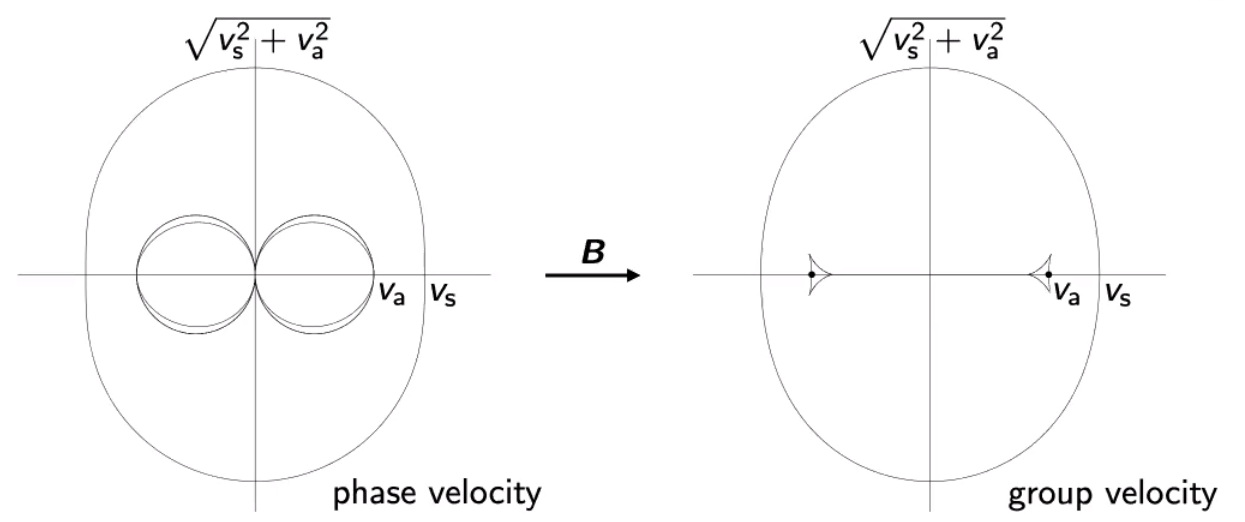
\includegraphics[width=0.7\textwidth]{friedrichs_2.png}
	\caption{Friedrichs diagram for the case $v_a < v_s$ ($v_a = 0.7 v_s$)}
	\label{fig:fd1}
\end{figure}
\begin{figure}
	\centering
	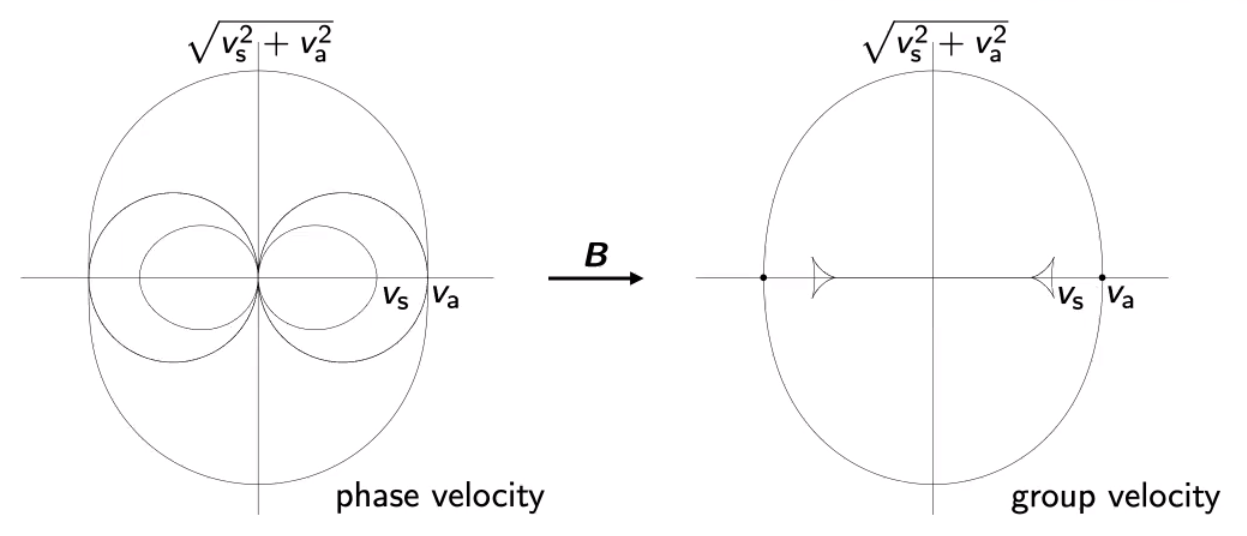
\includegraphics[width=0.7\textwidth]{friedrichs_1.png}
	\caption{Friedrichs diagram for the case $v_a > v_s$ ($v_s = 0.7 v_a$)}
	\label{fig:fd2}
\end{figure}

\paragraph{Interpretation.}
\begin{itemize}
	\item The fast wave is a quasi-isotropic acoustic-type wave in which both
		gas and magnetic pressure contribute.
	\item The slow wave is an acoustic-type wave that is strongly guided by
		$\B$.
	\item The Alfv\'{e}n wave is similar to a wave on an elastic string,
		propagating via magnetic tension and perfectly guided by $\B$.
\end{itemize}

\section{Non-linear waves, shocks and discontinuities}
\subsection{1D gas dynamics}
The equations of mass conservation and motion in 1D are
\begin{align}
	\frac{\partial \rho}{\partial t} + u \frac{\partial \rho}{\partial x} &= -
\rho \frac{\partial u}{\partial x}\\
	\frac{\partial u}{\partial t} + u \frac{\partial u}{\partial x} &= -
	\frac{1}{\rho}\frac{\partial p}{\partial x}
\end{align}
We assume the gas is homentropic ($s$ constant) and perfect. This eliminates
the entropy wave and leaves only the two sound waves. Then $p \propto
\rho^\gamma$ and $v_s^2 = \gamma p/\rho \propto \rho^{\gamma -1}$. We use
$v_s$ as a variable in place of $\rho$ or $p$:
\begin{equation}
	\diffd p = v_s^2\, \diffd \rho, \hspace{2em} \diffd \rho = \frac{\rho}{v_s}
	\frac{2 \,\diffd v_s}{\gamma -1}
\end{equation}
Then
\begin{align}
	\frac{\partial \rho}{\partial t} + u \frac{\partial \rho}{\partial x} +
	v_s \frac{\partial}{\partial x} \left( \frac{2v_s}{\gamma -1}\right)
	&= 0 \\
	\frac{\partial u}{\partial t} + u \frac{\partial}{\partial x}\left(\frac{2
v_s}{\gamma-1}\right) + v_s \frac{\partial u}{\partial x}&= 0
\end{align}
Add and subtract the two equations:
\begin{align}
	\left[ \frac{\partial}{\partial t} + (u+v_s)\frac{\partial}{\partial x}
	\right] \left( u + \frac{ 2 v_s}{\gamma -1}\right) &= 0 \\
	\left[ \frac{\partial}{\partial t} + (u-v_s)\frac{\partial}{\partial x}
	\right] \left( u - \frac{ 2 v_s}{\gamma -1}\right) &= 0 
\end{align}
Define the two \emph{Riemann invariants}
\begin{equation}
	R_\pm = u \pm \frac{2 v_s}{\gamma -1}
\end{equation}
Then we deduce that $R_\pm = \text{const.}$ along a \emph{characteristic
(curve)} $C_\pm$ of gradient
\begin{equation}
	\frac{\diffd x}{\diffd t} = u \pm v_s
\end{equation}
in the $(x,t)$ plane. The $\pm$ characteristics form an interlocking web
covering the space-time diagram. Both $R_+$ and $R_-$ are needed to
reconstruct the solution ($u$ and $v_s$). Half the information is propagated
along $C_+$ and half along $C_-$. In general $C_\pm$ are not known in advance
but must be determined along with the solution. $C_\pm$ propagate at speed
$v_s$ to the right and left, \emph{with respsect to the moving fluid}. This
may be viewed as a non-linear generalisation of the solution of the
classical wave equation $f(x-v_st) + g(x+v_s t)$.

\subsubsection{Method of characteristics}
Sketch of a numerical method of solution:
\begin{enumerate}
	\item Start with initial data ($u$ and $v_s$) for all relevant $x$ at
		$t=t_i$.
	\item Determine characteristic slopes at $t_i$.
	\item Propagate $R_\pm$ to $t=t_{i+1} = t_i + \delta t$, neglecting
		variation of characteristic slopes.
	\item Combine $R_\pm$ to find $u$ and $v_s$ at each $x$ at $t=t_{i+1}$.
	\item Re-evaluate slopes and repeat.
\end{enumerate}

\begin{center}
	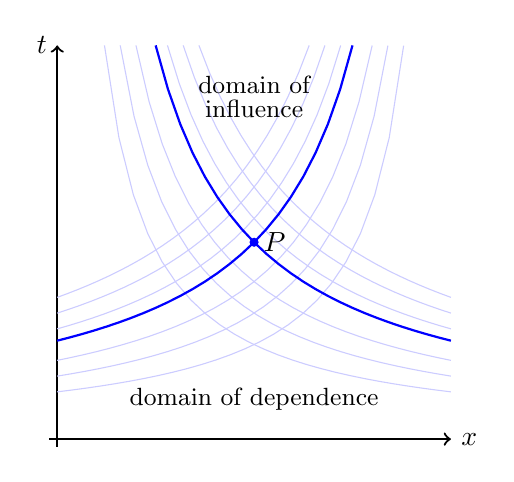
\begin{tikzpicture}
		\draw[thick,->] (-0.1, 0) -- (5, 0) node[right] {$x$};
		\draw[thick,->] (0, -0.1) -- (0, 5) node[left] {$t$};
		\draw[blue!20] plot[domain=1:5] ({\x},{5/\x});
		\draw[blue!20] plot[domain=0:4] ({\x},{-5/(\x-5)});
		\draw[blue!20] plot[domain=0.8:5] ({\x},{4/\x});
		\draw[blue!20] plot[domain=0:4.2] ({\x},{-4/(\x-5)});
		\draw[blue!20] plot[domain=0.6:5] ({\x},{3/\x});
		\draw[blue!20] plot[domain=0:4.4] ({\x},{-3/(\x-5)});
		\draw[blue!20] plot[domain=1.4:5] ({\x},{7/\x});
		\draw[blue!20] plot[domain=0:3.6] ({\x},{-7/(\x-5)});
		\draw[blue!20] plot[domain=1.6:5] ({\x},{8/\x});
		\draw[blue!20] plot[domain=0:3.4] ({\x},{-8/(\x-5)});
		\draw[blue!20] plot[domain=1.8:5] ({\x},{9/\x});
		\draw[blue!20] plot[domain=0:3.2] ({\x},{-9/(\x-5)});
		\draw[blue,thick] plot[domain=0:3.75] ({\x},{-6.25/(\x-5)});
		\draw[blue,thick] plot[domain=1.25:5] ({\x},{6.25/\x});
		\draw[blue,fill=blue] (2.5, 2.5) circle (0.05);
		\draw (2.5,2.5) node[right] {$P$};
		\draw (2.5, 4.5) node {\small domain of};
		\draw (2.5, 4.2) node {\small influence};
		\draw (2.5, 0.5) node {\small domain of dependence};
	\end{tikzpicture}
\end{center}

The \emph{domain of dependence} of a point $P$ in the spacetime diagram is the
region bounded by the $C_\pm$ through $P$ and located in the past of $P$. The
\emph{domain of influence} of $P$ is the region bounded by the $C_\pm$ through
$P$ and located in the future. The solution at $P$ cannot depend on anything
that occurs outside the domain of dependence. Similarly, the solution at $P$
cannot influence anything outside the domain of influence.

\subsubsection{A simple wave}
Suppose $R_-$ is uniform: the sme constant value on every $C_-$ characteristic
emanating from an undisturbed region to the right. Its value everywhere is
that of the undisturbed region:
\begin{equation}
	u - \frac{2 v_s}{\gamma -1} = u_0 - \frac{2v_{s0}}{\gamma -1}
\end{equation}
Then, along the $C_+$, both $R_\pm$ and so $u$ and $v_s$, are constant. The
$C_+$ therefore have constant slope $v = u+v_s$, so they are straight lines.
The statement that the wavespeed $v$ is constant along the family of straight
lines $\frac{\diffd x}{\diffd t} = v$ is expressed by the equation
\begin{equation}
	\frac{\partial v}{\partial t} + v \frac{\partial v}{\partial x} = 0
\end{equation}
known as the \emph{inviscid Burgers equation} or \emph{non-linear advection
equation}. 

This equation has only one set of characteristics, with slope
$\diffd x/\diffd t = v$, which is easily solved by the method of
characteristics. The initial data define $v_0(x) = v(x,0)$ and the
characteristics are straight lines. 

\begin{center}
	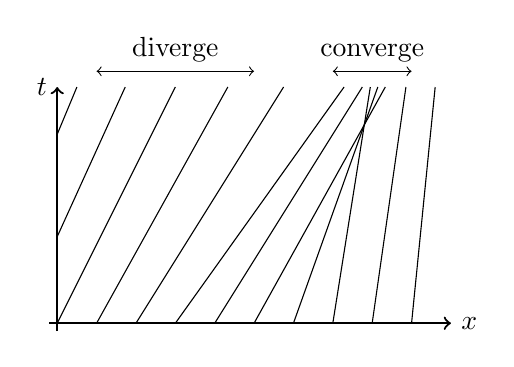
\begin{tikzpicture}
		\draw[thick,->] (-0.1, 0) -- (5, 0) node[right] {$x$};
		\draw[thick,->] (0, -0.1) -- (0, 3) node[left] {$t$};
		\draw plot[domain=1.1:3] ({-0.5+\x/2.2},{\x});
		\draw plot[domain=2.4:3] ({-1+\x/2.4},{\x});
		\draw plot[domain=0:3] ({\x/2},{\x});
		\draw plot[domain=0:3] ({0.5+\x/1.8},{\x});
		\draw plot[domain=0:3] ({1+\x/1.6},{\x});
		\draw plot[domain=0:3] ({1.5+\x/1.4},{\x});
		\draw plot[domain=0:3] ({2+\x/1.6},{\x});
		\draw plot[domain=0:3] ({2.5+\x/1.8},{\x});
		\draw plot[domain=0:3] ({3+\x/2.8},{\x});
		\draw plot[domain=0:3] ({3.5+\x/6.3},{\x});
		\draw plot[domain=0:3] ({4+\x/7},{\x});
		\draw plot[domain=0:3] ({4.5+\x/10},{\x});
		\draw[<->] (0.5, 3.2) -- (2.5, 3.2) node[midway,above] {diverge};
		\draw[<->] (3.5, 3.2) -- (4.5, 3.2) node[midway,above] {converge};
	\end{tikzpicture}
\end{center}

In regions where $\diffd v_0/\diffd x > 0$
the characteristics diverge in the future. In regions where $\diffd v_0/\diffd
x < 0$ the characteristics converge and will form a \emph{shock} at some
point. Contradictory information arrives at the same event, leading to a
breakdown of the solution.

\subsubsection{Wave steepening}
Another viewpoint of shock formation is \emph{wave steepening}. Each point of
the graph $v(x)$ moves at its wave speed $v$. The crest moves fastest and
eventually overtakes the trough to the right of it. 
\begin{figure}[h]
	\centering
	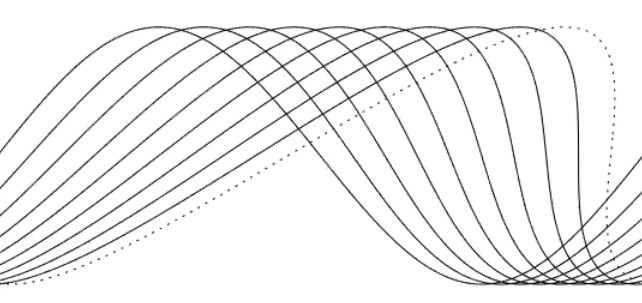
\includegraphics[width=0.3\textwidth]{steepening.png}
\end{figure}
The profile would become multiple-valued, but the wave breaks, forming a
discontinuity. The formal solution of the inviscid Burgers equation is
\begin{equation}
	v(x,t) = v_0(x_0)
\end{equation}
with $x = x_0 + v_0(x_0) t$. By the chain rule,
\begin{equation}
	\frac{\partial v}{\partial x} = \frac{v_0'}{1+v_0' t}
\end{equation}
which diverges first at the breaking time
\begin{equation}
	t^* = \frac{1}{\max(-v_0')}
\end{equation}

\subsection{Simple non-linear waves}
Recall the hyperbolic structure of the equations:
\begin{equation}
	\frac{\partial \symbf{U}}{\partial t} + \symsf{A}_i \frac{\partial
	\symbf{U}}{\partial x_i} = 0, \hspace{2em} \symbf{U} = \left[ \rho, p, \u,
	\B\right]^T
\end{equation}
These are hyperbolic because the eigenvalues of $\symsf{A}_i n_i$ are real for
any unit vector $n_i$. The eigenvalues are wave speeds, eigenvectors are
wave modes.

In a simple wave propagating in the $x$-direction, all physical quantities are
functions of a single variable, the phase $\psi(x,t)$. Then $\symbf{U} =
\symbf{U}(\psi)$ and so
\begin{equation}
	\frac{\diffd \symbf{U}}{\diffd \psi}\frac{\partial \psi}{\partial t} +
	\symsf{A}_x \frac{\diffd \symbf{U}}{\diffd \psi} \frac{\partial
	\psi}{\partial x} = 0
\end{equation}
This equation is satisfied if $\diffd \symbf{U}/\diffd \psi$ is an eigenvector
of the hyperbolic system and if
\begin{equation}
	\frac{\partial \psi}{\partial t} + v \frac{\partial \psi}{\partial x} = 0
\end{equation}
where $v$ is the corresponding wave speed (eigenvalue). But since $v =
v(\psi)$ we again find
\begin{equation}
	\frac{\partial v}{\partial t}+ v \frac{\partial v}{\partial x} = 0
\end{equation}
which is the inviscid Burgers equation.  Steepening is therefore generic for
simple waves, but waves do not always steepen in practice. For example, linear
dispersion arising from Coriolis or buoyancy forces can counteract nonlinear
wave steepening. Waves propagating on a non-uniform background are not simple
waves. Waves may be damped by diffusive processes (viscosity, thermal
conduction or resistivity) before they can steepen. 

Even some simple waves do not steepen. This happens if the wave
speed $v$ does not depend on the variables that actually vary in the wave
mode, for which there are two simple examples: the entropy wave ($v = u_x$) in
which $\rho$ varies but not $p$ or $u_x$. Also, the Alfv\'{e}n wave ($v=u_x
\pm v_{ax}$) in which $u_y, u_z, B_y, B_z$ vary but not $\rho, p, u_x, B_x$.
In these cases the relevant solution of the inviscid Burgers equation is just
$v = \text{const.}$ The slow and fast magnetoacoustic waves, though, are
`generally nonlinear' and undergo steepening.

\subsection{Shocks \& discontinuities}
\subsubsection{Jump conditions}
Discontinuities are resolved by diffusive processes (viscosity, thermal
conduction or resistivity) that become more important on smaller length
scales. We could solve the non-ideal (M)HD equations to resolve the internal
structure of a shock. This internal solution could be matched onto external
solutions in which diffusion is neglected. However, the matching conditions
can be determined from conservation laws without resolving internal structure.

Consider a shock front at rest at $x=0$ (make a Galilean transformation if
necessary). Look for a stationary, 1D solution (equivalent to assuming a
separation of scales) in which gas flows from left to right.

\begin{center}
	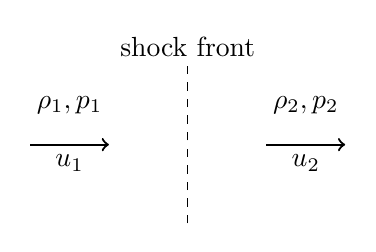
\begin{tikzpicture}
		\draw[dashed] (0,0) -- (0, 2) node[above] {shock front};
		\draw[thick,->] (-2, 1) -- (-1, 1) node[midway, below] {$u_1$};
		\draw[thick,->] (1, 1) -- (2, 1) node[midway, below] {$u_2$};
		\draw (-1.5, 1.5) node {$\rho_1, p_1$};
		\draw (1.5, 1.5) node {$\rho_2, p_2$};
	\end{tikzpicture}
\end{center}

On the left is upstream, pre-shock material ($\rho_1, p_1$, etc.) and on the
right is downstream, post-shock material ($\rho_2, p_2$, etc.) Consider any
equation in conservative form
\begin{equation}
	\frac{\partial q}{\partial t} + \nabla \cdot \symbf{F} = 0
\end{equation}
For a stationary, 1D solution, $F_x$ is constant. Write the matching condition
as
\begin{equation}
	\dif{F_x} = F_{x,2} - F_{x,1} = 0
\end{equation}
Including non-ideal effects gives rise to additional diffusive fluxes (not of
mass but of momentum, energy, magnetic flux, etc.) The diffusive fluxes are
negligible outside the shock, so they do not affect the jump conditions. This
is valid as long as the new physics does not introduce any source terms in the
equations. So the total energy is a properly conserved quantity, \emph{but not
the entropy} (see later). 

Consider the conservative form of the momentum equation:
\begin{equation}
	\frac{\partial}{\partial t}(\rho u_i) + \nabla \cdot \left(\rho u_i \u + \Pi
	\symbf{e}_i - \frac{B_i \B}{\mu_0}\right) = 0
\end{equation}
Including gravity makes no difference to the jump conditions because $\Phi$ is
continuous (it satisfies $\nabla^2 \Phi = 4\pi G \rho$). From mass
conservation, we have
\begin{equation}
	\dif{\rho u_x} = 0
\end{equation}
From momentum conservation:
\begin{align}
	\dif{\rho u_x^2 + \Pi - \frac{B_x^2}{\mu_0}} &= 0 \\
	\dif{\rho u_x u_y + \Pi - \frac{B_x B_y}{\mu_0}} &= 0 \\
	\dif{\rho u_x u_z + \Pi - \frac{B_x B_z}{\mu_0}} &= 0
\end{align}
From the solenoidal condition $\nabla \cdot \B = 0$:
\begin{equation}
	\dif{B_x} =0 
\end{equation}
From the induction equation $\B_t + \nabla \times \symbf{E} = 0$:
\begin{align}
	\dif{u_x B_y - u_y B_x} = -\dif{E_z} &= 0 \\
	\dif{u_x B_z - u_z B_x} = \dif{E_y} &= 0
\end{align}
These are the standard electromagnetic relations at an interface: continuity
of $\bot$ component of $\B$ and $\parallel$ components of $\symbf{E}$. From
total energy conservation:
\begin{equation}
	\dif{\rho u_x\left(\frac{1}{2}u^2 + h\right) + \frac{1}{\mu_0}(E_yB_z -
	E_z B_y)} = 0
\end{equation}
Although the entropy in ideal MHD satisfies an equation of conservative form,
\begin{equation}
	\frac{\partial}{\partial t}(\rho s) + \nabla \cdot (\rho s \u) = 0
\end{equation}
the dissipation of energy within the shock provides a source term for entropy.
The entropy flux is \emph{not} continuous across the shock.

\subsubsection{Non-magnetic shocks}
First consider a \emph{normal shock} ($u_y = u_z = 0$) with no magnetic field.
We obtain the \emph{Rankine-Hugoniot relations}
\begin{align}
	\dif{\rho u_x} &= 0\\
	\dif{\rho u_x^2 + p} &= 0\\
	\dif{\rho u_x\left(\frac{1}{2}u_x^2 +h\right)} &= 0
\end{align}
The specific enthalpy of a perfect gas is
\begin{equation}
	h = \frac{\gamma}{\gamma -1}\frac{p}{\rho}
\end{equation}
The analytical solution is derived in example sheet 3. Introduce the upstream
Mach number (the \emph{shock Mach number}):
\begin{equation}
	\M_1 = \frac{u_{x1}}{v_{s1}} > 0
\end{equation}
where $v_{s1}$ is the upstream adiabatic sound speed. Then we find
\begin{align}
	\frac{u_{x1}}{u_{x2}} = \frac{\rho_2}{\rho_1} &=
	\frac{(\gamma+1)\M_1^2}{(\gamma-1)\M_1^2 + 2} \\
	\frac{p_2}{p_1} &= \frac{2\gamma \M_1^2 - (\gamma-1)}{\gamma +1}\\
	\M_2^2 &= \frac{2+(\gamma-1)\M_1^2}{2\gamma M_1^2 - (\gamma -1)}
\end{align}
Note that $\rho_2/\rho_1$ and $p_2/p_1$ are increasing functions of $\M_1$.
The case $\M_1 = \M_2 = 1$ is trivial (no shock): $\rho_2/\rho_1 = 1$,
$p_2/p_1 = 1$. Two cases exist in general:
\begin{itemize}
	\item \emph{Compression shock}
		\begin{equation}
			\M_1 > 1, \hspace{2em} \M_2 < 1, \hspace{2em} \rho_2 > \rho_1,
			\hspace{2em} p_2 > p_1
		\end{equation}
	\item \emph{Rarefaction shock}
		\begin{equation}
			\M_1 < 1, \hspace{2em} \M_2 > 1, \hspace{2em} \rho_2 < \rho_1,
			\hspace{2em} p_2 < p_1
		\end{equation}
\end{itemize}
The entropy change $\dif{s}$ in passing through the shock is positive for
compression shocks and negative for rarefaction shocks (see ES3, Q1).
Therefore only compression shocks are physically realisable; rarefaction
shocks are excluded by the second law of thermodynamics. All shocks involve
dissipation and irreversibility.  The fact that $\M_1 > 1$ while $\M_2 < 1$
means the shock travels supersonically relative to the upstream gas and
subsonically relative to the downstream gas.

\begin{itemize}
	\item In the \emph{weak shock} limit $\M_1 - 1 \ll 1$ the relative
		velocity of the fluid and the shock is close to the sound speed on
		both sides.
	\item In the \emph{strong shock} limit $\M_1 \gg 1$, common in
		astrophysical applications,
		\begin{align}
			\frac{u_{x1}}{u_{x2}} = \frac{\rho_2}{\rho_1} &\to \frac{\gamma +
			1}{\gamma -1} \\
				\frac{p_2}{p_1} &\gg 1 \\
				\M_2^2 &\to \frac{\gamma -1}{2 \gamma}
		\end{align}
\end{itemize}
Note that the compression ratio $\rho_2/\rho_1$ is finite (and equal to $4$
when $\gamma = 5/3$). In the rest frame of the undisturbed (upstream) gas the 
\emph{shock speed} is $u_{\text{sh}} = -u_{x1}$. The downstream density,
velocity (in that frame) and pressure in the limit of a strong shock are (to
be used in section 7)
\begin{align}
	\rho_2 &= \left(\frac{\gamma +1}{\gamma -1}\right) \rho_1 \\
	u_{x2} - u_{x1} &= \frac{2u_{\text{sh}}}{\gamma +1} \\
	p_2 &= \frac{2 \rho_1 u_{\text{sh}}^2}{\gamma +1}
\end{align}

A lot of thermal energy is generated out of kinetic energy by a strong shock:
\begin{equation}
	e_2 = \frac{2 u_{\text{sh}}^2}{(\gamma+1)^2}
\end{equation}

\subsubsection{Oblique shocks}
When $u_y$ or $u_z$ is non-zero, we also require
\begin{equation}
	\dif{\rho u_x u_y} = \dif{\rho u_x u_z} = 0
\end{equation}
Since $\rho u_x$ is continuous across the shock (and non-zero), we deduce that
$\dif{u_y} = \dif{u_z} = 0$. Momentum and energy conservation apply as before,
and we recover the Rankine-Hugoniot relations.

\subsubsection{Other discontinuities}
The discontinuity is not called a shock if there is no normal flow ($u_x =0$).
In this case we can deduce only that $\dif{p} = 0$. Arbitrary discontinuities
are allowed in $\rho, u_y$ and $u_z$. These are related to the entropy and
vortical waves. A jump in $\rho$ is a \emph{contact discontinuity} and a jump
in $u_y$ or $u_z$ is a \emph{tangential discontinuity} or \emph{vortex sheet}
(vorticity proportional to $\delta(x)$). These discontinuities are not
produced naturally by wave steepening, because the entropy and vortical waves
do not steepen. However they do appear in the Riemann problem (see later) and
other situations with discontinuous initial conditions.

\subsubsection{MHD shocks and discontinuities}
When a magnetic field is included, the jump conditions allow a wider variety
of solutions. There are different types of discontinuity associated with the
three MHD waves (Alfv\'{e}n, slow and fast), which we will not discuss here.
Since the parallel components of $\B$ need not be continuous, it is pssible
for them to `switch on' or `switch off' on passage through a shock. 

A \emph{current sheet} is a tangential discontinuity in the magnetic field.
For example, suppose $B_y$ changes sign across the interface, with $B_x = 0$.
Then the current density $J_z \propto \delta(x)$.

\subsubsection{The Riemann problem}
The Riemann problem is a fundamental initial value problem for a hyperbolic
system and plays a central role in some numerical methods for solving the
equations of AFD.

The initial condition at $t=0$ consists of two uniform states separated by a
discontinuity at $x=0$. In the case of 1D gas dynamics, we have
\begin{equation}
	\rho = \begin{cases} \rho_L & x < 0 \\ \rho_R & x > 0 \end{cases}
	\hspace{2em}
	p = \begin{cases} p_L & x < 0 \\ p_R & x > 0 \end{cases}
	\hspace{2em}
	u_x = \begin{cases} u_L & x < 0 \\ u_R & x > 0 \end{cases}
\end{equation}

An example is the `shock tube' problem in which gas at different pressure is
at rest either side of a partition which is released at $t=0$. It can be shown
that the initial discontinuity resolves generically into three simple waves.
The inner one is a contact discontinuity. The other ones are shocks or
rarefaction waves (see below).

The initial data define no natural length-scale, but they do allow a
characteristic velocity scale $c$ to be defined (although not uniquely). The
result is a \emph{similarity solution} in which variables depend on $x$ and
$t$ only through the dimensionless combination $\xi = x/ct$. 

Unlike the physical rarefaction shock, the \emph{rarefaction wave} (or
\emph{expansion wave}) is a non-dissipative, homentropic, continuous simple
wave in which $\nabla \cdot \u > 0$. If we seek a similarity solution $v =
v(\xi)$ of the inviscid Burgers equation $v_t + vv_x = 0$ we find $v=x/t$ (or
the trivial solution $v = \text{const}$). The characteristics form an
\emph{expansion fan}.

\begin{center}
	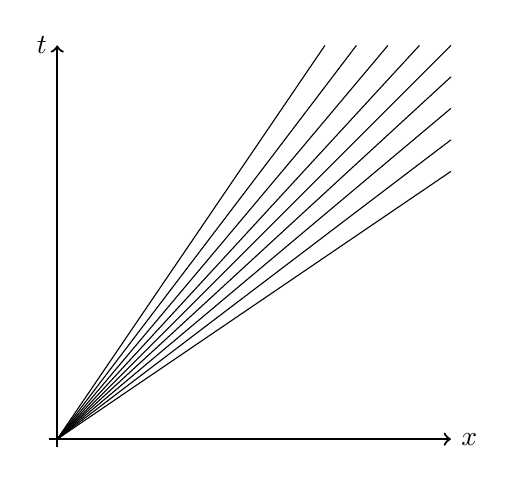
\begin{tikzpicture}
		\draw[thick,->] (-0.1, 0) -- (5, 0) node[right] {$x$};
		\draw[thick,->] (0, -0.1) -- (0, 5) node[left] {$t$};
		\draw (0,0) -- (5, 5);
		\draw (0,0) -- (5, 4.6);
		\draw (0,0) -- (5, 4.2);
		\draw (0,0) -- (5, 3.8);
		\draw (0,0) -- (5, 3.4);
		\draw (0,0) -- (4.6, 5);
		\draw (0,0) -- (4.2, 5);
		\draw (0,0) -- (3.8, 5);
		\draw (0,0) -- (3.4, 5);
	\end{tikzpicture}
\end{center}

The `+' rarefaction wave has
\begin{equation}
	u+v_s = \frac{x}{t}, \hspace{2em} R_- = u - \frac{2 v_s}{\gamma -1} =
	\text{const.}
\end{equation}
determined by the undisturbed right-hand state. The `-' rarefaction wave has
\begin{equation}
	u-v_s = \frac{x}{t}, \hspace{2em} R_+ = u + \frac{2 v_s}{\gamma -1} =
	\text{const.}
\end{equation}
determined by the undisturbed left-hand state.  In each case $u$ and $v_s$ are
linear functions of $x/t$ and
\begin{equation}
	\nabla \cdot \u = \left(\frac{2}{\gamma +1}\right)\frac{1}{t} > 0
\end{equation}
A typical outcome of a shock-tube problem consists of (from left to right):
undisturbed region, rarefaction wave, uniform region, contact discontinuity,
uniform region, shock, undisturbed region.

\begin{center}
	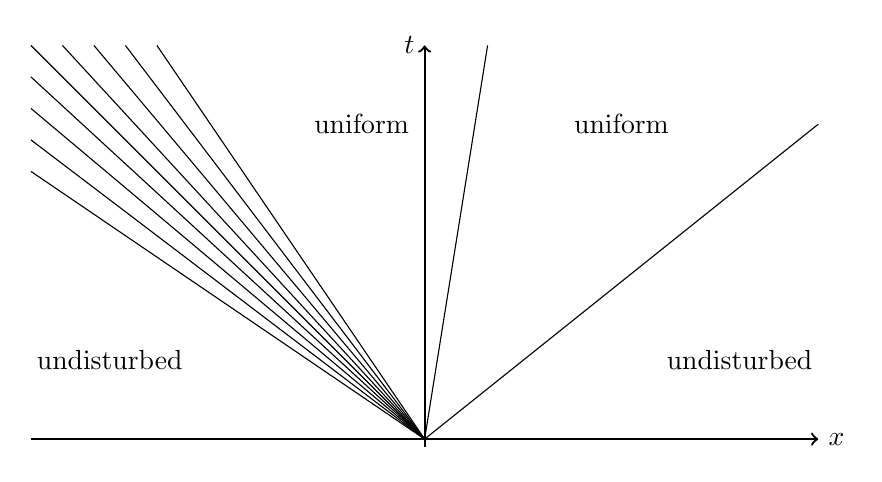
\begin{tikzpicture}
		\draw[thick,->] (-5, 0) -- (5,0) node[right] {$x$};
		\draw[thick,->] (0, -0.1) -- (0, 5) node[left] {$t$};
		\draw (0,0) -- (5, 4);
		\draw (0,0) -- (0.8, 5);
		\draw (0,0) -- (-3.4, 5);
		\draw (0,0) -- (-3.8, 5);
		\draw (0,0) -- (-4.2, 5);
		\draw (0,0) -- (-4.6, 5);
		\draw (0,0) -- (-5, 5);
		\draw (0,0) -- (-5, 4.6);
		\draw (0,0) -- (-5, 4.2);
		\draw (0,0) -- (-5, 3.8);
		\draw (0,0) -- (-5, 3.4);
		\draw (4, 1) node {undisturbed};
		\draw (2.5, 4) node {uniform};
		\draw (-0.8, 4) node {uniform};
		\draw (-4, 1) node {undisturbed};
	\end{tikzpicture}
\end{center}

In Godunov's method and related algorithms, the equations of AFD are advanced
in time by solving (either exactly or approximately) a Riemann problem at each
cell boundary.

\section{Spherical blast waves: supernovae}
\subsection{Introduction}
In this section $(r, \theta, \phi)$ are spherical polar coordinates. In a
supernova, an energy of order $10^{51}$ erg ($10^{44}$ J) is released into the
interstellar medium. An expanding spherical blast wave is formed as the
explosion sweeps up the surrounding gas. Several good examples of these
supernova remnants are observed in the galaxy, e.g. Tycho's supernova of 1572
and Kepler's supernova of 1604.

\begin{figure}
	\centering
	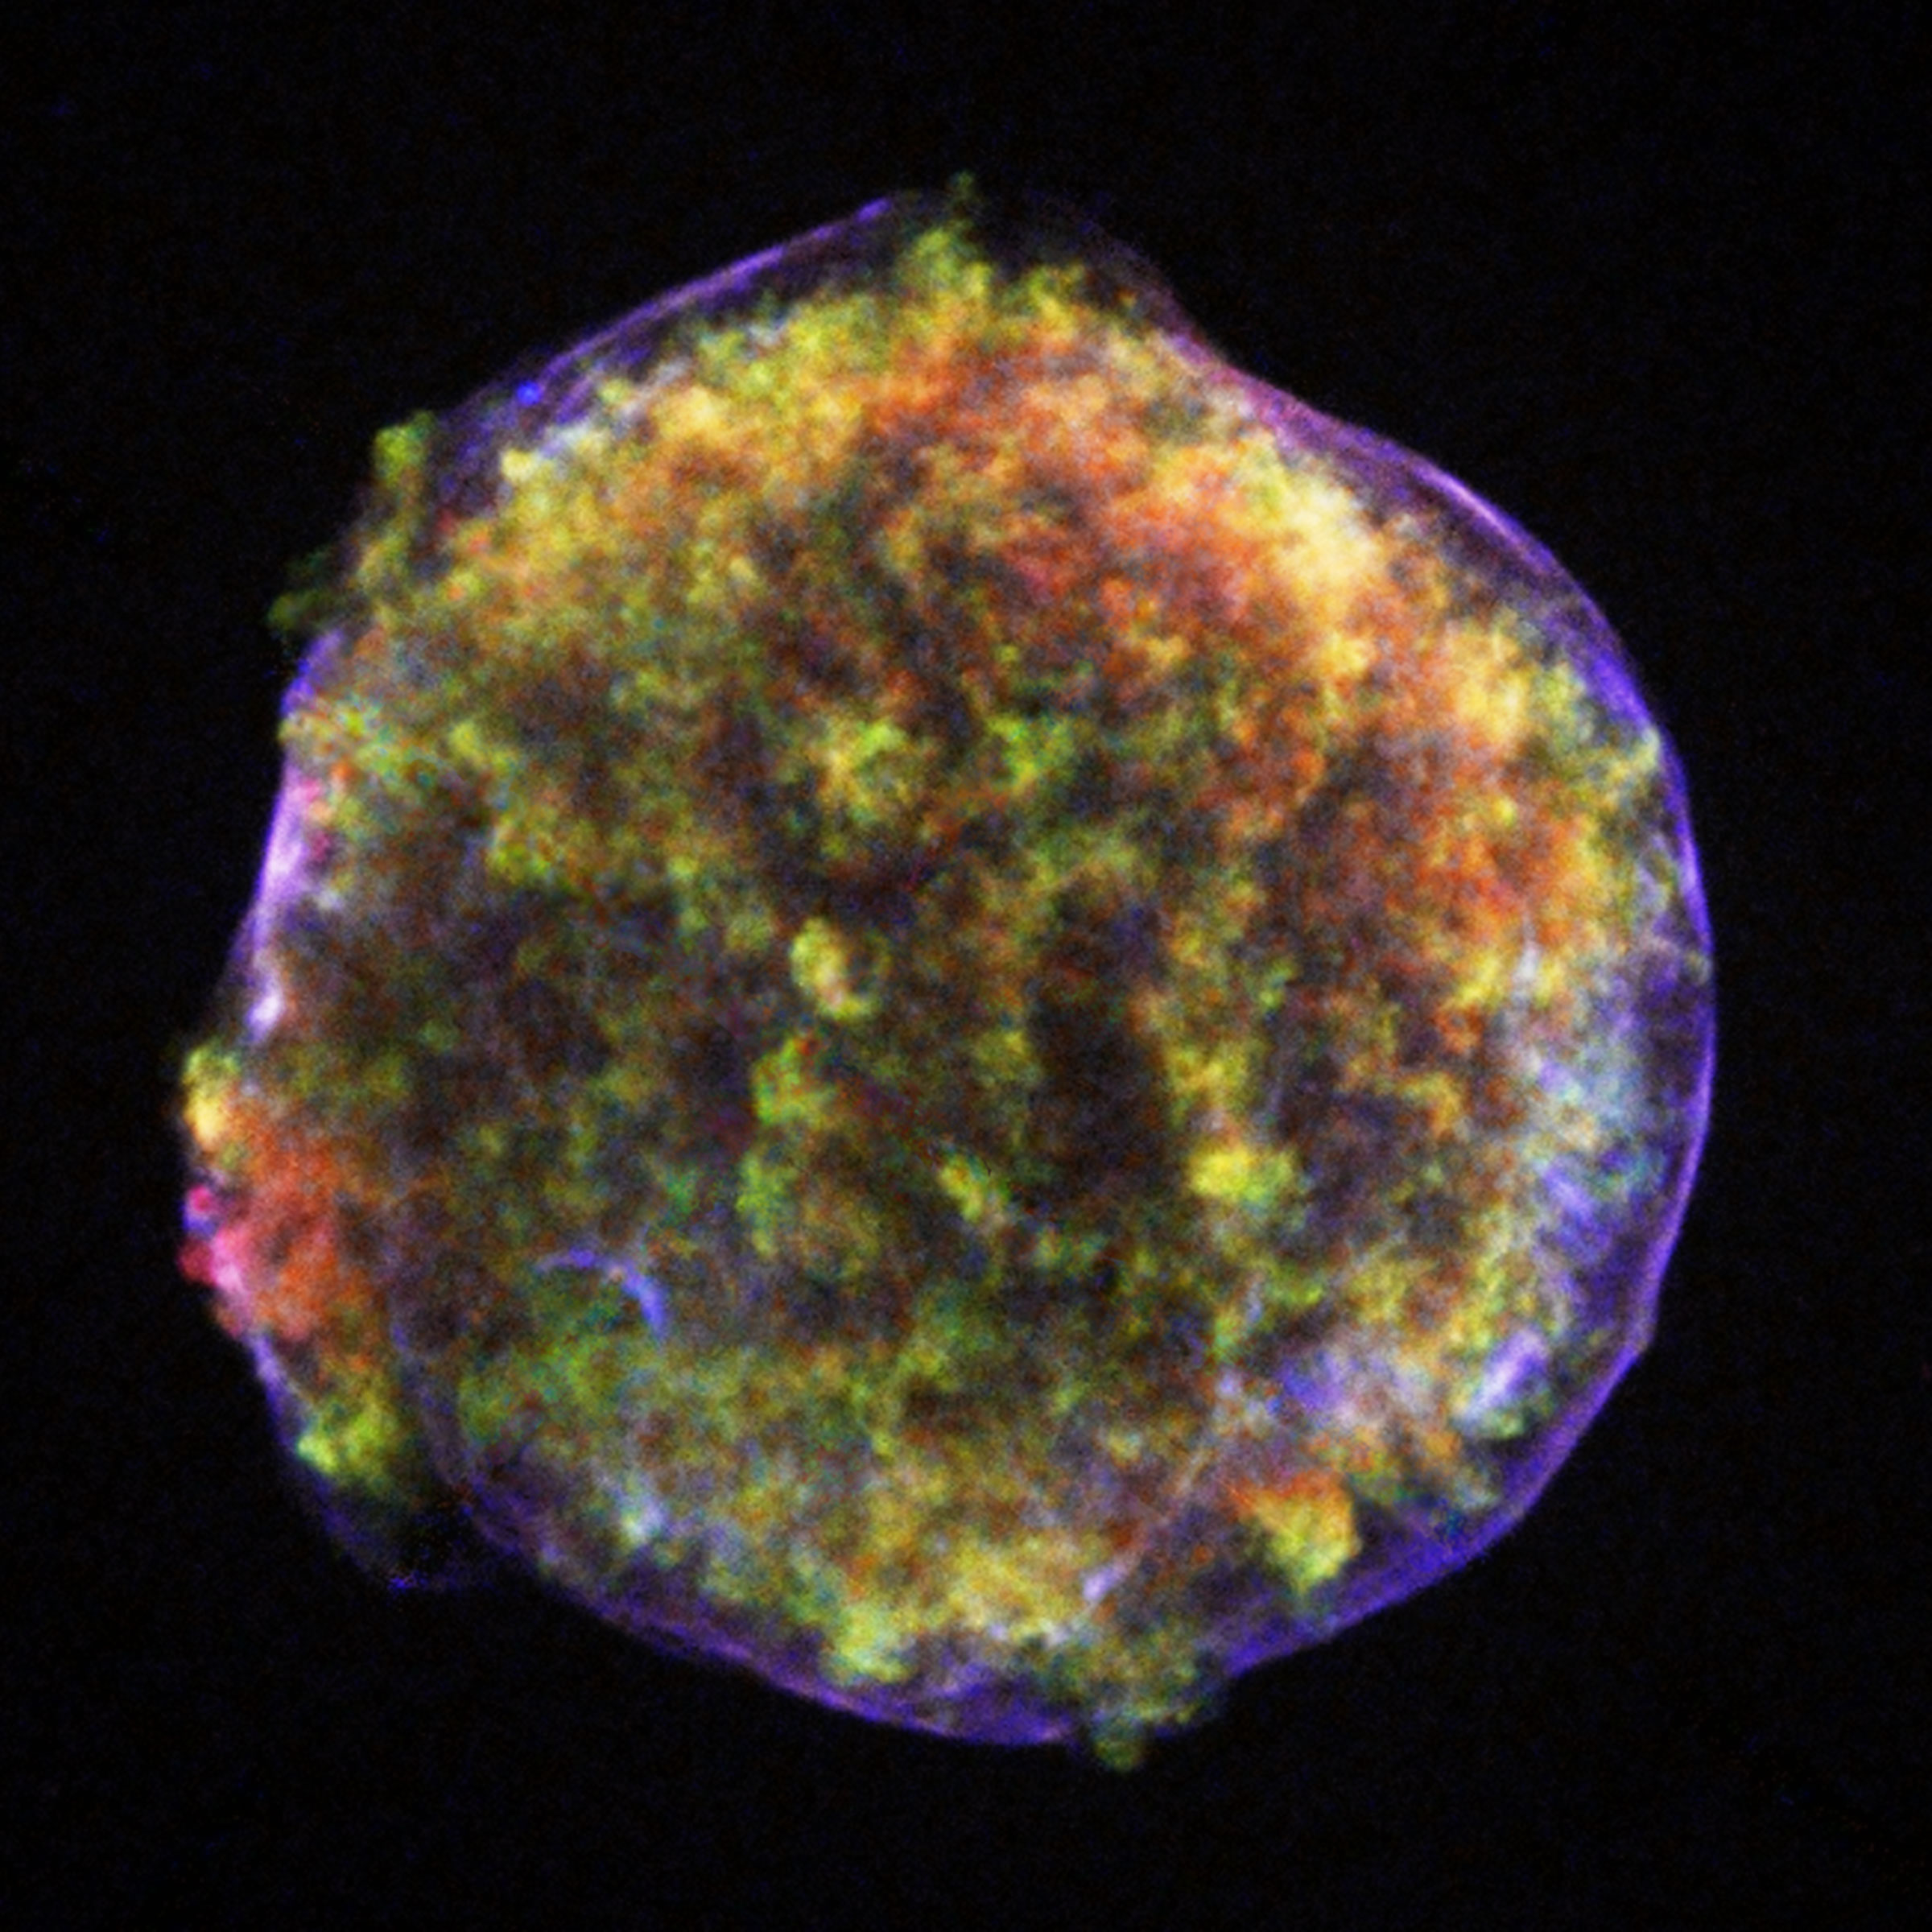
\includegraphics[width=0.5\textwidth]{sn1572.jpg};
	\caption{Tycho's supernova, SN1572. Source: Wikipedia.}
\end{figure}

The effect is similar to a bomb. Photographs of the first atomic bomb test in
New Mexico in 1945 allowed both Sedov in the Soviet Union and Taylor in the UK
to work out the bomb's energy ($20$ kt of TNT $\sim 10^{14}$ J). 

Suppose an energy $E$ is released at $t=0, r=0$ and that the explosion is
spherically symmetric. The external medium has density $\rho_0$ and pressure
$p_0$. In the \emph{Sedov-Taylor phase} of the explosion, the pressure $p \gg
p_0$. Then a strong shock is formed and the external pressure $p_0$ can be
neglected (formally set to zero). Gravity is also negligible in the dynamics.

\subsection{Governing equations}
A spherically symmetric flow of a perfect gas with purely radial velocity $u_r
= u(r,t)$ satisfies
\begin{align}
\left( \frac{\partial}{\partial t} + u \frac{\partial}{\partial r}\right)\rho
&= -\frac{\rho}{r^2} \frac{\partial}{\partial r} (r^2 u) \label{eq:l13:1} \\
\left( \frac{\partial}{\partial t} + u \frac{\partial}{\partial r}\right)u
&= -\frac{1}{\rho} \frac{\partial p}{\partial r} \label{eq:l13:2} \\
\left( \frac{\partial}{\partial t} + u \frac{\partial}{\partial r}\right) \ln
	(p \rho^{-\gamma}) &= 0 \label{eq:l13:3}
\end{align}
which are the equations of mass continuity, momentum conservation and energy
conservation. These imply the total energy equation
\begin{equation}
	\frac{\partial}{\partial t}\left(\frac{1}{2}\rho u^2 + \frac{p}{\gamma
	-1}\right) + \frac{1}{r^2} \frac{\partial}{\partial r} \left[ r^2 \left(
	\frac{1}{2}\rho u^2 + \frac{\gamma p}{\gamma -1}\right)u\right] = 0
	\label{eq:l13:energy}
\end{equation}

The shock is at $r=R(t)$ so the shock speed is $\dot{R}$. The equations are to
be solved in $0 < r < R$ with the strong shock conditions at $r=R$:
\begin{align}
	\rho &= \frac{\gamma+1}{\gamma-1} \rho_0 \label{eq:l13:4}\\
	u&= \frac{2 \dot{R}}{\gamma +1}\label{eq:l13:5}\\
	p &= \frac{2\rho_0 \dot{R}^2}{\gamma +1} \label{eq:l13:6}
\end{align}
which are the Rankine-Hugoniot conditions in the limit of a strong shock. The
total energy of the explosion is
\begin{equation}
	E = \int_0^R \left( \frac{1}{2}\rho u^2 + \frac{p}{\gamma -1}\right) 4\pi
	r^2 \, \diffd r = \text{const.}
\end{equation}
The thermal energy of the external medium is negligible.

\subsection{Dimensional analysis}
The dimensional parameteres of the problem on which the solution might depend
are $E$ and $\rho_0$. Their dimensions are
\begin{equation}
	\left[E\right] = M L^2 T^{-2}, \hspace{2em} \left[ \rho_0\right] = M
	L^{-3}
\end{equation}
Together, they do not define a characteristic lengthscale, so the explosion is
`scale-free' or `self-similar'. If the dimensional analysis includes the time
$t$ since the explosion, however, we can find a time-dependent characteristic
lengthscale. The radius of the shock must be
\begin{equation}
	R = \alpha \left( \frac{E t^2}{\rho_0}\right)^{1/5}
\end{equation}
where $\alpha$ is a dimensionless constant to be determined.

\subsection{Similarity solution}
Self-similarity is expressed using the dimensionless \emph{similarity
variable} $\xi = r/R(t)$.  The solution has the form
\begin{equation}
	\rho = \rho_0 \tilde{\rho}(\xi), \hspace{2em} u = \dot{R} \tilde{u}(\xi),
	\hspace{2em} p = \rho_0 \dot{R}^2 \tilde{p}(\xi)
\end{equation}
where $\tilde{\rho}, \tilde{u}$ and $\tilde{p}$ are dimensionless functions of
$\xi$ to be determined. 

Meaning: the graph of $u$ versus $r$, for example, has a constant shape but
both axes of the graph are rescaled as time proceeds and the shock expands.

\subsection{Dimensionless equations}
Substitute the known forms $\rho = \rho_0 \tilde{\rho}, u = \dot{R} \tilde{u},
p = \rho_0 \dot{R}^2 \tilde{p}$ into \eqref{eq:l13:1}, \eqref{eq:l13:2},
\eqref{eq:l13:3} and cancel dimensionless factors to get
\begin{align}
	(\tilde{u}-\xi) \tilde{\rho}' &= - \frac{\tilde{\rho}}{\xi^2}
	\frac{\diffd}{\diffd \xi}(\xi^2 \tilde{u}) \label{eq:l13:7}\\
	(\tilde{u}-\xi)\tilde{u}' - \frac{3}{2}\tilde{u} &=
	-\frac{\tilde{p}'}{\tilde{\rho}} \label{eq:l13:8}\\
	(\tilde{u}-\xi)\left(\frac{\tilde{p}'}{\tilde{p}} - \frac{\gamma
\tilde{\rho}'}{\tilde{\rho}}\right) -3 &= 0\label{eq:l13:9}
\end{align}
This uses $\dot{R} \propto t^{-3/5}, \xi \propto R t^{-2/5}$. The strong shock
conditions \eqref{eq:l13:4}, \eqref{eq:l13:5}, \eqref{eq:l13:6} at $r=R$ imply
\begin{equation}
	\tilde{\rho} = \frac{\gamma+1}{\gamma-1}, \hspace{2em} \tilde{u} =
	\frac{2}{\gamma +1}, \hspace{2em} \tilde{p} = \frac{2}{\gamma +1}
	\label{eq:l13:BCs}
\end{equation}
at $\xi = 1$. The total energy integral becomes a normalisation condition
\begin{equation}
	1 = \frac{16 \pi}{25} \alpha^5 \int_0^1 \left(
	\frac{1}{2}\tilde{\rho}\tilde{u}^2 + \frac{\tilde{p}}{\gamma -1}\right)
	\xi^2\, \diffd \xi
\end{equation}
that will determine the value of $\alpha$.

\subsection{First integral}
The total energy equation \eqref{eq:l13:energy} is in 1D conservative form 
\begin{equation}
	\frac{\partial q}{\partial t} = \frac{\partial F}{\partial r} = 0
	\label{eq:l14:1}
\end{equation}
with
\begin{align}
	q &= r^2 \left( \frac{1}{2} \rho u^2 + \frac{p}{\gamma -1}\right) \\
	F &= r^2 \left( \frac{1}{2} \rho u^2 + \frac{\gamma p}{\gamma -1} \right)
	u
\end{align}

For the similarity solution, we have
\begin{equation}
	q = \rho_0 R^2 \dot{R}^2 \tilde{q}(\xi), \hspace{2em} F = \rho_0 R^2
	\dot{R}^3 \tilde{F}(\xi) \label{eq:l14:2}
\end{equation}
with
\begin{align}
	\tilde{q} &= \xi^2 \left( \frac{1}{2}\tilde{\rho}\tilde{u}^2 +
	\frac{\tilde{p}}{\gamma -1}\right) \label{eq:l14:3}\\
	\tilde{F} &= \xi^2 \left( \frac{1}{2}\tilde{\rho}\tilde{u}^2 +
	\frac{\gamma \tilde{p}}{\gamma -1}\right) \tilde{u}\label{eq:l14:4}
\end{align}
Substitute \eqref{eq:l14:2} into \eqref{eq:l14:1}, noting that $R^2 \dot{R}^2
\propto t^{4/5} t^{-6/5} \propto t^{-2/5} \propto R^{-1}$:
\begin{align}
	\rho_0 R^2 \dot{R}^2 \left[ -\frac{\dot{R}}{R} \tilde{q} + \frac{\diffd
	\tilde{q}}{\diffd \xi} \left( -\frac{\dot{R}}{R} \xi \right) +
	\frac{\dot{R}}{R} \frac{\diffd \tilde{F}}{\diffd \xi}\right] &= 0 \\
	\implies -\tilde{q} - \xi \frac{\diffd \tilde{q}}{\diffd xi} +
	\frac{\diffd \tilde{F}}{\diffd \xi} &= 0  \\
	\implies \frac{\diffd}{\diffd \xi} \left( \tilde{F} - \xi \tilde{q}\right)
									   &= 0
\end{align}
Hence $\tilde{F} - \xi \tilde{q} = \text{const.} = 0$ for a solution that is
finite at $\xi = 0$. Using \eqref{eq:l14:3} and \eqref{eq:l14:4}, solve
$\tilde{F} - \xi \tilde{q} = 0$ for $\tilde{p}$:
\begin{equation}
	\tilde{p} = \frac{(\gamma - 1)\tilde{\rho}\tilde{u}^2(\xi -
	\tilde{u})}{2(\gamma \tilde{u} - \xi)}
\end{equation}
This is compatible with the boundary conditions at $\xi = 1$ expressed by
\eqref{eq:l13:BCs}. Having found a first integral, we can dispense with the
thermal energy equation \eqref{eq:l13:9}. Let $\tilde{u} = v \xi$. We now have
from \eqref{eq:l13:7} and \eqref{eq:l13:8}:
\begin{align}
	(v-1)\frac{\diffd \ln \tilde{\rho}}{\diffd \ln \xi} &= -\frac{\diffd
	v}{\diffd \ln \xi} - 3v \\
	(v-1) \frac{\diffd v}{\diffd \ln \xi} + \frac{1}{\tilde{\rho}\xi^2}
	\frac{\diffd}{\diffd \ln \xi} \left[ \frac{(\gamma -1)\tilde{\rho} \xi^2
	v^2 (1-v)}{2(\gamma v-1)}\right] &= \frac{3}{2}v
\end{align}
Eliminate $\tilde{\rho}$:
\begin{equation}
	\frac{\diffd v}{\diffd \ln \xi} = \frac{v(\gamma v -
		1) \left[5-(3\gamma-1)v\right]}{\gamma (\gamma+1) v^2 - 2(\gamma +1)v
	+ 2}
\end{equation}
Invert and split into partial fractions:
\begin{equation}
\frac{\diffd \ln \xi}{\diffd v} = -\frac{2}{5v} + \frac{\gamma(\gamma
	-1)}{(2\gamma +1)(\gamma v - 1)} + \frac{13\gamma^2 -7\gamma +
	12}{5(2\gamma +1)\left[5-(3\gamma -1)v\right]}
\end{equation}
The solution is
\begin{equation}
	\xi \propto v^{-2/5} (\gamma v-1)^{(\gamma -1)/(2\gamma +1)}
	\left[5-(3\gamma-1)v\right]^{-(13\gamma^2-7\gamma+12)/5(2\gamma
	+1)(3\gamma -1)}
\end{equation}
Then
\begin{align}
	\frac{\diffd \ln \tilde{\rho}}{\diffd v} &= -\frac{1}{v-1} -
	\frac{3v}{v-1}\frac{\diffd \ln \xi}{\diffd v}  \\
	&= \frac{2}{(2-\gamma)(1-v)} + \frac{3\gamma}{(2\gamma+1)(\gamma v-1)} -
	\frac{13\gamma^2 - 7\gamma +12}{(2-\gamma)(2\gamma+1) \left[5-(3\gamma
	-1)v\right]}
\end{align}
The solution is
\begin{equation}
	\tilde{\rho} \propto (1-v)^{-2/(2-\gamma)}(\gamma
	v-1)^{3/(2\gamma+1)}\left[5-(3\gamma-1)v\right]^{
	(13\gamma^2-7\gamma+12)/(2-\gamma)(2\gamma
	+1)(3\gamma -1)}
\end{equation}
For example, with $\gamma =5/3$:
\begin{align}
	\xi &\propto v^{-2/5} \left(\frac{5v}{3}-1\right)^{2/13}
	\left(5-4v\right)^{-82/195} \\
	\tilde{\rho} &\propto
	(1-v)^{-6}\left(\frac{5v}{3}-1\right)^{9/13}(5-4v)^{82/13}
\end{align}
To satisfy $v=2/(\gamma+1) = 3/4$ and $\tilde{\rho} = (\gamma+1)/(\gamma-1) =
4$ at $\xi = 1$ we have
\begin{align}
	\xi &= \left(\frac{4v}{3}\right)^{-2/5} \left(\frac{20v}{3}-4\right)^{2/13}
	\left(\frac{5}{2}-2v\right)^{-82/195} \\
	\tilde{\rho} &=
	4(4-4v)^{-6}\left(\frac{20v}{3}-4\right)^{9/13}(\frac{5}{2}-2v)^{82/13}
\end{align}
Then, from the first integral
\begin{equation}
	\tilde{p} =
	\frac{3}{4}\left(\frac{4v}{3}\right)^{6/5}(4-4v)^{-5}\left(\frac{5}{2}-2v\right)^{82/15}
\end{equation}

\begin{figure}[h]
	\centering
	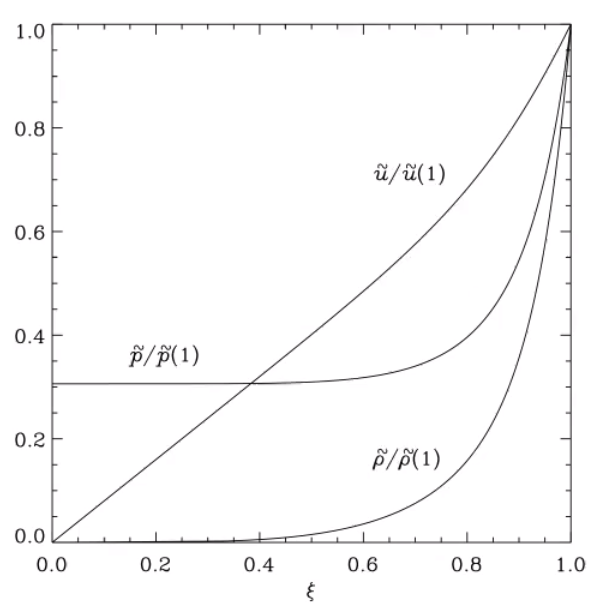
\includegraphics[width=0.4\textwidth]{supernova.png}
	\caption{Normalised solutions for $0 \le \xi \le 1$ with $\gamma =5/3$.}
\end{figure}
In this solution, $\xi$ ranges from 0 to 1, and $v$ from $3/5$ to $3/4$. The
normalisation integral (numerically) gives $\alpha \approx 1.152$.

\subsection{Applications}
Some rough estimates from the above analysis:
\begin{itemize}
	\item For a supernova, $E \sim 10^{51}$ erg and $\rho_0 \sim 10^{-24}
		\text{g}\cdot\text{cm}^{-3}$. Then $R \approx 6$pc and $\dot{R} \approx
		2000 \text{km}\cdot\text{s}^{-1}$ at $t=1000$yr.
	\item For the 1945 New Mexico explosion, $E \approx 8 \times 10^{20}$ erg,
		$\rho_0 \approx 1.2 \times 10^{-3} \text{g}\cdot\text{cm}^{-3}$. Then
		$R \approx 100$m and $\dot{R} \approx 4 \text{km}\cdot\text{s}^{-1}$
		at $t=0.01$s.
\end{itemize}

The similarity method is useful in a wide range of nonlinear problems. In this
case it reduced PDEs to integrable ODEs.

\end{document}
